\input{../../common/slide-common-header.tex}

\newcommand{\orgNum}{0}
\newcommand{\orgTopic}{org meeting}
\newcommand{\orgKey}{syllabus, contacts}

\newcommand{\introNum}{1}
\newcommand{\introTopic}{introduction to multithreading}
\newcommand{\introKey}{concurrency, parallelism, agents, threads, scheduler, Amdahl's law, race condition, deadlock, wait-for graph}

\newcommand{\basicNum}{2}
\newcommand{\basicTopic}{basic concepts}
\newcommand{\basicKey}{mutex, acquisition order, reentrancy, fairness, data locking, code locking, signalling, condition variable, lost signal, spurious wakeup}

\newcommand{\syncPrimitivesNum}{3}
\newcommand{\syncPrimitivesTopic}{advanced synchronization primitives}
\newcommand{\syncPrimitivesKey}{monitor, latch, barrier, thundering herd, semaphore, read-write lock, thread pool, executor, producer-consumer, fork-join, load balancing}

\newcommand{\patternsNum}{4}
\newcommand{\patternsTopic}{advanced synchronization concepts}
\newcommand{\patternsKey}{interruption, cancellation, partitioning, privatization, replication, thread-local, ownership}

\newcommand{\extraBasicsNum}{5}
\newcommand{\extraBasicsTopic}{additional topics of practical concurrency}
\newcommand{\extraBasicsKey}{documenting protocols and classes, checking concurrent invariants, stress testing, execution trace analysis, estimating required testing effort, static and dynamic checks, scheduling randomization, model checking}

\newcommand{\foundationsNum}{6}
\newcommand{\foundationsTopic}{theoretical foundations of concurrency}
\newcommand{\foundationsKey}{timeline, partial order, sequential consistency, linearizability, quiscent consistency, correctness, liveness, safety, atomicity}

\newcommand{\foundationsPlusNum}{7}
\newcommand{\foundationsPlusTopic}{progress guarantees, concurrent operations hierarchy, consensus number}
\newcommand{\foundationsPlusKey}{obstruction-free, lock-free, wait-free, safe register, regular register, atomic register, consensus number, register snapshots}

\newcommand{\atomicsNum}{8}
\newcommand{\atomicsTopic}{introduction to atomics}
\newcommand{\atomicsKey}{compare-and-swap, fetch-and-add, spinning, lock-free stack, taxonomy of queues, ABA problem}

\newcommand{\cacheCoherencyNum}{9}
\newcommand{\cacheCoherencyTopic}{cache coherency}
\newcommand{\cacheCoherencyKey}{cache memory hierarchy, cache coherency protocol. store-buffer, load-buffer, invalidate-queue, memory barrier, hardware memory model, weak memory model, litmus tests}

\newcommand{\langMMNum}{10}
\newcommand{\langMMTopic}{language memory model}
\newcommand{\langMMKey}{motivation, approaches, comparison of existing solutions}

\newcommand{\advancedConcurrencyNum}{11}
\newcommand{\advancedConcurrencyTopic}{advanced concurrency}
\newcommand{\advancedConcurrencyKey}{CLH/MCS queue/lock, backoff policies revisited, notify-as-ready, RAT optimization, single LIFO cell optimization, work distribution, work stealing, taxonomy of parallel problems}

\newcommand{\userSpaceThreadingNum}{12}
\newcommand{\userSpaceThreadingTopic}{user-space threading}
\newcommand{\userSpaceThreadingKey}{berkley socket, blocking and non-blocking IO, callback-hell, async-await, continuation-passing-style, fibers/coroutines/green threads, stackful vs stackless}


\newcommand{\designNum}{13}
\newcommand{\designTopic}{designing concurrent systems}
\newcommand{\designKey}{park/unpark, synchronizer, futex/wait-on-address, plan9 approach, race-finders, ForkJoinPool/CoroutineCarriers/UIthread, observability, structured concurrency}

\newcommand{\frameworksAndDistributedNum}{14}
\newcommand{\frameworksAndDistributedTopic}{multi-agent systems}
\newcommand{\frameworksAndDistributedKey}{auto-parallelization languages and frameworks, semi-automatic synchronization, distributed systems, consensus protocols}


\title[]{Lecture \foundationsNum: \foundationsTopic}
\subtitle[]{\foundationsKey}
\author[]{Alexander Filatov\\ filatovaur@gmail.com}

\date{}

\begin{document}

\begin{frame}
  \titlepage
  \url{https://github.com/Svazars/parallel-programming/blob/main/slides/pdf/l6.pdf}
\end{frame}

\begin{frame}{In previous episodes}

Concurrency is complicated due to:
\begin{itemize}
  \item Independence of agents 
  \begin{itemize}
    \item combinatorial explosion of possible executions
  \end{itemize}
  \item Uncontrollable execution speed of agents 
  \begin{itemize}
    \item spurious failures
  \end{itemize}  
  \item Uncertainty with definition of consistency 
  \begin{itemize}
    \item concurrent invariants
    \item visibility
    \item data race
    \item atomicity
  \end{itemize}  
\end{itemize}

\pause

Is it purely engineering issue or we have encountered some fundamental problem?

\end{frame}


\begin{frame}{Be patient}

Reminder: you are studying Turing Machines or Finite-State Machines in order to
\begin{itemize}
  \item get a compact and fully formalized description of some "computing device"
  \item understand theoretical limitations of an object (Halting Problem, Pumping Lemma)
\end{itemize}

\pause

It usually takes several mathematically-intensive sessions to go from the definition to really interesting theorems.

\pause

Concurrency is more "inherently-complicated" \ so it takes even more time to rigorously prove non-trivial properties. 

\pause

We will skip or simplify some steps.

\pause
There still will be a lot of technical (yet mathematically heavy) parts. 

\pause
At least, you will understand why proving concurrent algorithms could be really hard. 

\end{frame}

\begin{frame}{Supplementary materials}

\begin{itemize}
  \item Chapters 1-5 in "The Art of Multiprocessor Programming" 
  \item Companion materials \url{https://booksite.elsevier.com/9780123973375}
\end{itemize}

Our course briefly introduces some important theoretical concepts, for better understanding consider looking through
\begin{itemize}
  \item \texttt{chapter\_02.ppt}
  \item \texttt{chapter\_03.ppt}  
\end{itemize}

\end{frame}


\begin{frame}{Theoretical mode enabled}

\textbf{Important:} in Lecture~\foundationsNum \ (today) and Lecture~\foundationsPlusNum \ (next time) we will use \textbf{pseudo}code.

\pause

It looks like Java and feels like Java but algorithms from the slides \textbf{will not work} as expected if run on the JVM. 

\pause

In Lecture~\cacheCoherencyNum \ and Lecture~\langMMNum \ we will understand why.

\pause

We are going to do some real Computer Science, it should work from mathematical point of view ;)

\pause

Theoretical intuition and insights will help us to understand how to implement efficient and correct algorithms using existing hardware.

\pause

\textbf{Hint:} focus on ideas rather mathematical formalisms.

\end{frame}


\begin{frame}{Lecture plan}
\tableofcontents
\end{frame}

\section{Time, events, intervals, precedence}


\begin{frame}[fragile, t]{Time and events}

An \textbf{event} $a_0$ of thread \texttt{A} is
\begin{itemize}
  \item Instantaneous
  \item No simultaneous events (break ties)
\end{itemize}

\begin{center}
  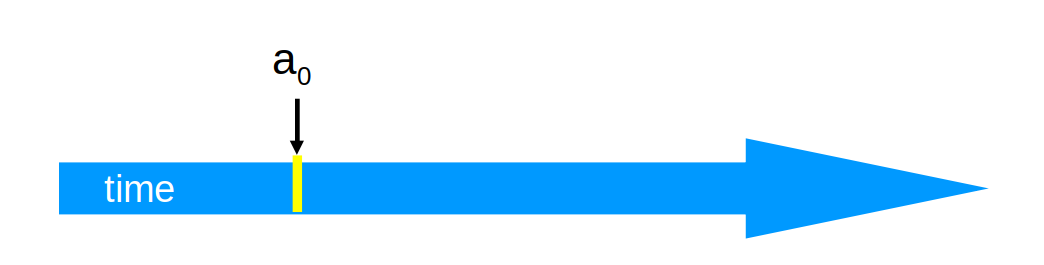
\includegraphics[width=0.5\textwidth]{./pics/time/Timeline.png}
\end{center}

\end{frame}


\begin{frame}[fragile, t]{Threads}

A thread \texttt{A} is (formally) a sequence $a_0$, $a_1$, ... of events 
\begin{itemize}
  \item “Trace” model
  \item Notation: $a_0 \rightarrow a_1$ indicates order
\end{itemize}

\begin{center}
  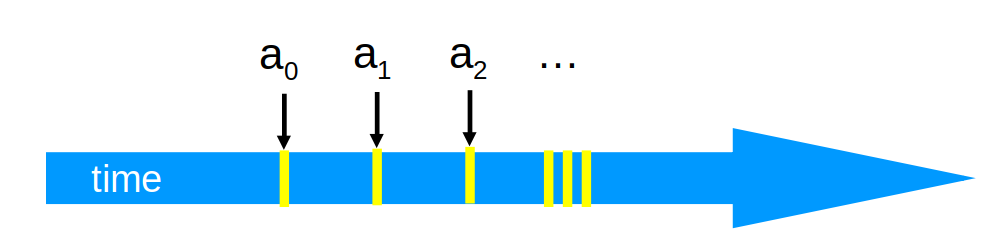
\includegraphics[width=0.5\textwidth]{./pics/time/ThreadTrace.png}
\end{center}

\pause
Example Thread events:
\begin{itemize}
  \item Assign to shared or local variable
  \item Invoke method
  \item Return from method
  \item ...
\end{itemize}

\end{frame}

\begin{frame}[fragile, t]{Threads are state machines}

\begin{center}
  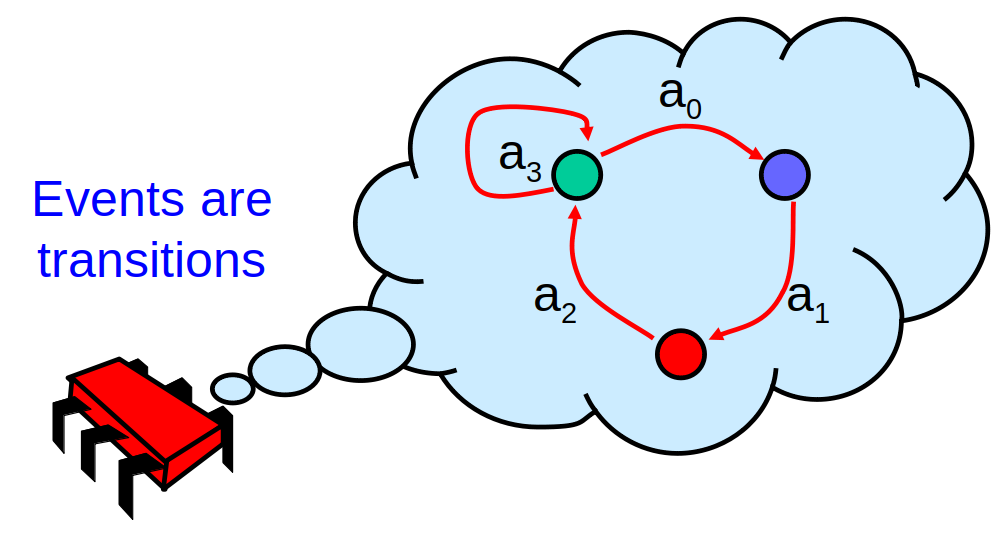
\includegraphics[width=0.7\textwidth]{./pics/time/ThreadsStateMachines.png}
\end{center}

\end{frame}


\begin{frame}[fragile]{Concurrent threads}

\begin{tabular}{p{7cm}p{5cm}}
\textcolor{yellow}{Thread A}  & \textcolor{green}{Thread B} \\
\begin{center}
  
\includegraphics[width=0.4\textwidth]{./pics/time/ThreadA.png}
\end{center}
&
\begin{center}
  
\includegraphics[width=0.4\textwidth]{./pics/time/ThreadB.png}
\end{center}

\end{tabular}

Events of two or more threads:
\begin{itemize}
  \item Interleaved
  \item Not necessarily independent
\end{itemize}
\begin{center}
  
\includegraphics[width=0.5\textwidth]{./pics/time/Interleavings.png}
\end{center}

\end{frame}

\begin{frame}[fragile]{Methods are intervals}

An \textbf{interval}  $A_0 =(a_0, a_1)$ is
\begin{itemize}
  \item Time between events $a_0$ and $a_1$ 
\end{itemize}

\begin{center}
  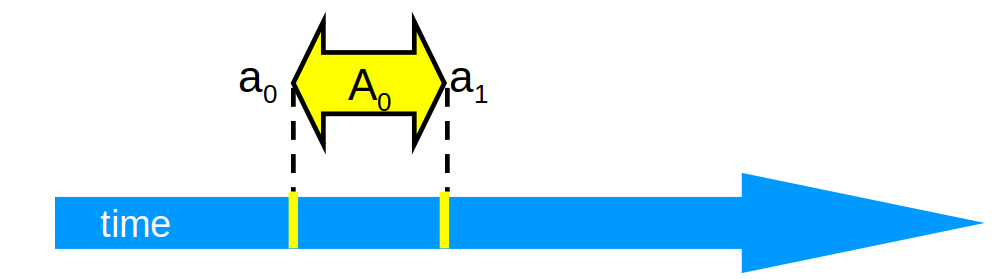
\includegraphics[width=0.5\textwidth]{./pics/time/Interval.png}
\end{center}
\end{frame}

\begin{frame}[fragile]{Overlapping intervals}

\begin{center}
  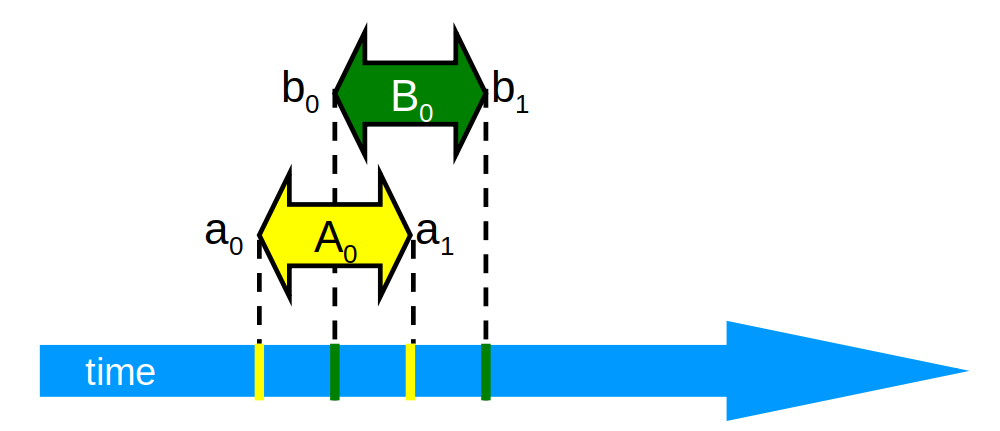
\includegraphics[width=0.5\textwidth]{./pics/time/Overlap.png}
\end{center}

\end{frame}


\begin{frame}[fragile]{Disjoint intervals}
\begin{center}
  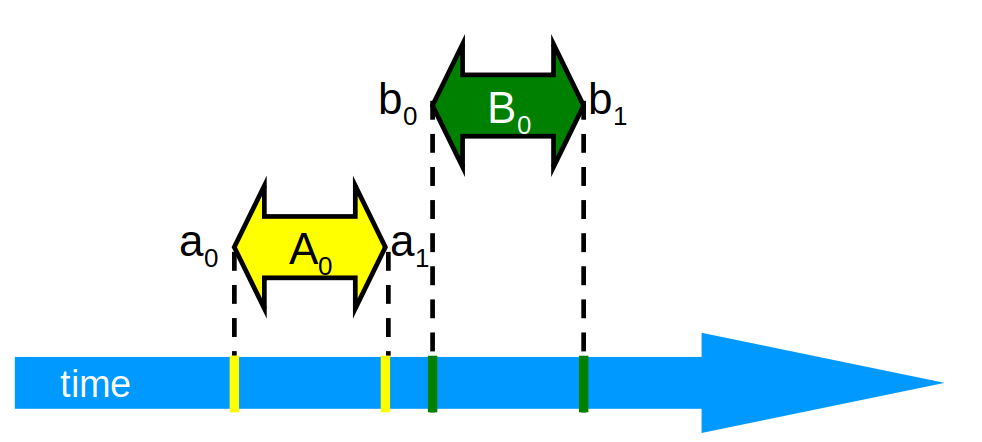
\includegraphics[width=0.5\textwidth]{./pics/time/Disjoint.png}
\end{center}

\pause
\textbf{Precedence}:
\begin{itemize}
  \item Interval $A_0$ \textbf{precedes} interval $B_0$
  \item Notation: $A_0 \rightarrow B_0$
\end{itemize}

\end{frame}


\begin{frame}[fragile]{Precedence}

$A_0 \rightarrow B_0$
\begin{itemize}
  \item $A_0$ \textbf{precedes} interval $B_0$
  \pause
  \item $A_0$ \textbf{happens before} interval $B_0$
  \pause
  \item Fancy way to say "Middle Ages $\rightarrow$ Renaissance"
\end{itemize}

\pause

what about \textit{this week} vs \textit{this month}?

\pause

\onslide<7->{Precedence is a partial order}:
\begin{itemize}
  \item Never true that $A \rightarrow A$. \onslide<8->{(Irreflexive)}
  \item If $A \rightarrow B$ then not true $B \rightarrow A$.  \onslide<9->{(Antisymmetric)}
  \item If $A \rightarrow B$ and $B \rightarrow C$ then $A \rightarrow C$. \onslide<10->{(Transitive)}
  \pause
  \item Remember: $A \rightarrow B$ and $B \rightarrow A$ might both be false!
\end{itemize}

\end{frame}



\section{Mutual exclusion}
\showTOC

\subsection{2 threads}

\begin{frame}{Mutual exclusion}

Thread is \textit{well formed} if:
\begin{itemize}
  \item each critical section is associated with a unique \texttt{Lock} object
  \item \texttt{Lock.lock} when trying to enter critical section
  \item \texttt{Lock.unlock} when leaving critical section
\end{itemize}

Let $CS_{A}^{j}$ be the interval: thread \texttt{A} executes critical section for \texttt{j}-th time.

\end{frame}

\begin{frame}{Mutual exclusion for 2 agents}

$CS_{A}^{j}$: thread \texttt{A} executes critical section for \texttt{j}-th time.

\pause

\textbf{Mutual exclusion}:
\begin{itemize}
  \item Critical sections of different threads do not overlap. \pause
   $\forall A, B, k, j \ CS_{A}^{k} \rightarrow CS_{B}^{j}$ or $CS_{B}^{j} \rightarrow CS_{A}^{k}$
\end{itemize}

\pause
\textbf{Freedom from deadlock}:
\begin{itemize}
  \item If some thread attempts to acquire the lock, then some thread will succeed in acquiring the lock. If thread \texttt{A} calls \texttt{lock()}
  but never acquires the lock, then other threads must be completing an infinite number of critical sections.
\end{itemize}

\pause

\textbf{Freedom from starvation (lockout freedom)}:
\begin{itemize}
  \item Every thread that attempts to acquire the lock eventually succeeds. Every call to \texttt{lock()} eventually returns.
\end{itemize}

\pause

\begin{theorem}
  Starvation freedom implies deadlock freedom.
\end{theorem} 
\end{frame}

\questiontime{Mutual exclusion, Freedom from deadlock, Freedom from starvation. Which are safety properties, which are liveness properties?}

\questiontime{Restaurant "Concurrency pitfalls" \ claims that every philosopher will eat ordered meal before Sun explodes. Does it provide \textbf{Freedom from starvation}?}


\begin{frame}[fragile]{LockOne}

\begin{minted}{java}
class LockOne implements Lock {
  boolean[] flag = new boolean[2];
  void lock() {
    int i = ThreadID.get(); // 0 or 1
    int j = 1 - i;
    flag[i] = true;         // I want to enter
    while (flag[j]) {}      // await other thread
  }
  void unlock() {
    int i = ThreadID.get();  
    flag[i] = false;        // I do not want to enter any more
  }
}
\end{minted}
\end{frame}

\begin{frame}[fragile]{LockOne: deadlock}

\begin{minted}{java}
void lock() {
  int i = ThreadID.get();
  int j = 1 - i;
  flag[i] = true;
  while (flag[j]) {}
}
void unlock() {
  flag[ThreadID.get()] = false;
}
\end{minted}

$write_{A}(flag[A] = true)$ occur before $read_{B}(flag[A])$

$write_{B}(flag[B] = true)$ occur before $read_{A}(flag[B])$
\end{frame}


\begin{frame}[fragile]{LockOne: mutual exclusion}
\begin{minted}{java}
void lock() {
  flag[i] = true;
  while (flag[j]) {}
}
void unlock() {
  flag[i] = false;
}
\end{minted}

From the code:
\begin{itemize}
  \item $write_{A}(flag[A] = true) \rightarrow read_{A}(flag[B] = false) \rightarrow CS_{A}$ 
  \item $write_{B}(flag[B] = true) \rightarrow read_{B}(flag[A] = false) \rightarrow CS_{B}$ 
\end{itemize}

\end{frame}


\begin{frame}[fragile]{LockOne: mutual exclusion}

Plan:
\begin{itemize}
  \item Assume $CS_A^j$ overlaps $CS_B^k$.
  \item Consider each thread's last ($j$-th and $k$-th) read and write in the \texttt{lock()} method before entering 
  \item Derive a contradiction
\end{itemize}

\pause
Informal hint: Thread A observed \texttt{flag[B] = false} and entered $CS_A^j$ \textbf{and then} Thread B entered $CS_B^k$ which required to write \texttt{flag[B] = true}

\pause
From assumption:
\begin{itemize}
  \item $read_{A}(flag[B] = false) \rightarrow write_{B}(flag[B] = true)$ 
  \item $read_{B}(flag[A] = false) \rightarrow write_{A}(flag[A] = true)$ 
\end{itemize}

\end{frame}

\begin{frame}[fragile]{LockOne: mutual exclusion}
\begin{center}
  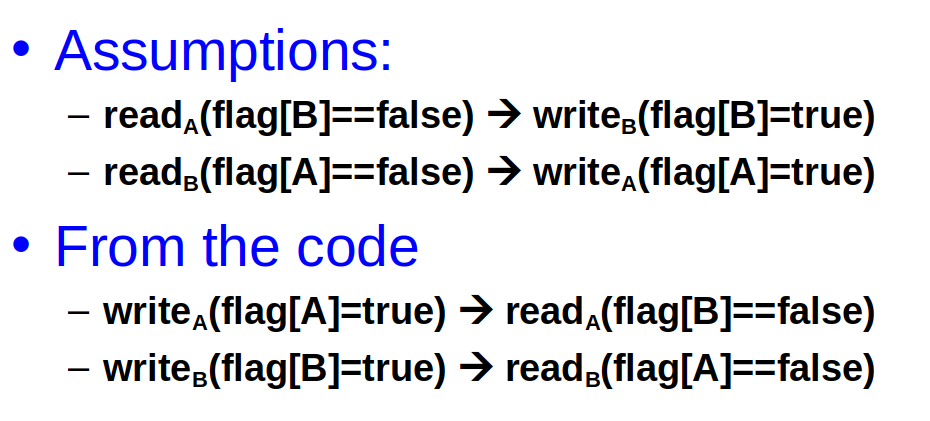
\includegraphics[width=0.8\textwidth]{./pics/lock1/combine-1.png}
\end{center}
\end{frame}

\begin{frame}[fragile,nofrmanumbering]{LockOne: mutual exclusion}
\begin{center}
  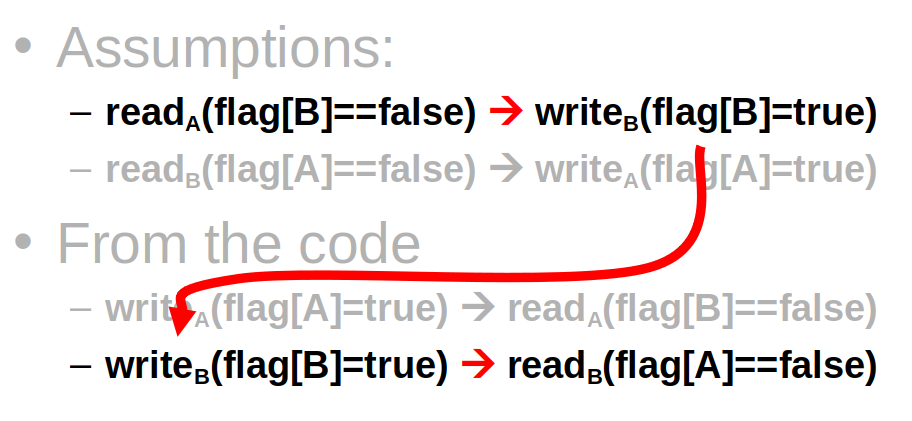
\includegraphics[width=0.8\textwidth]{./pics/lock1/combine-2.png}
\end{center}
\end{frame}

\begin{frame}[fragile,nofrmanumbering]{LockOne: mutual exclusion}
\begin{center}
  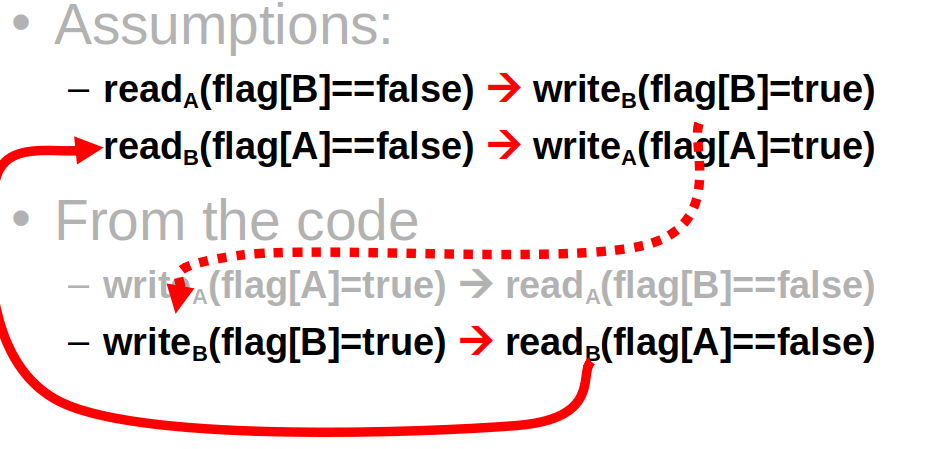
\includegraphics[width=0.8\textwidth]{./pics/lock1/combine-3.png}
\end{center}
\end{frame}

\begin{frame}[fragile,nofrmanumbering]{LockOne: mutual exclusion}
\begin{center}
  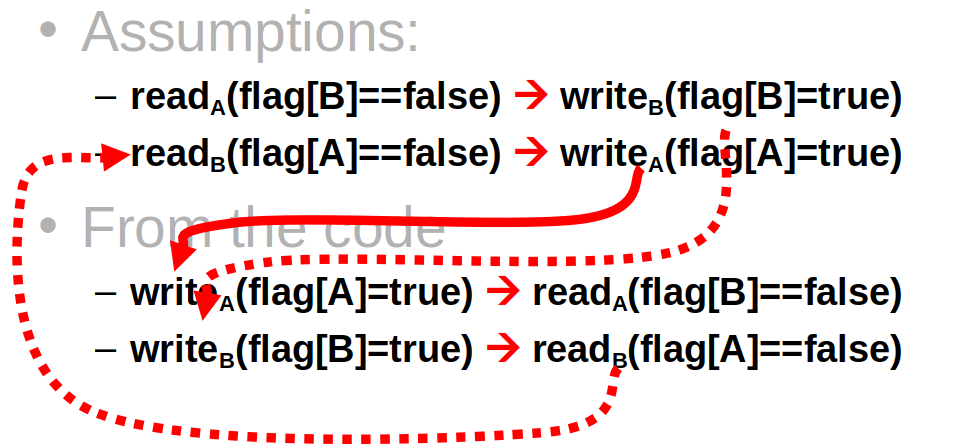
\includegraphics[width=0.8\textwidth]{./pics/lock1/combine-4.png}
\end{center}
\end{frame}

\begin{frame}[fragile,nofrmanumbering]{LockOne: mutual exclusion}
\begin{center}
  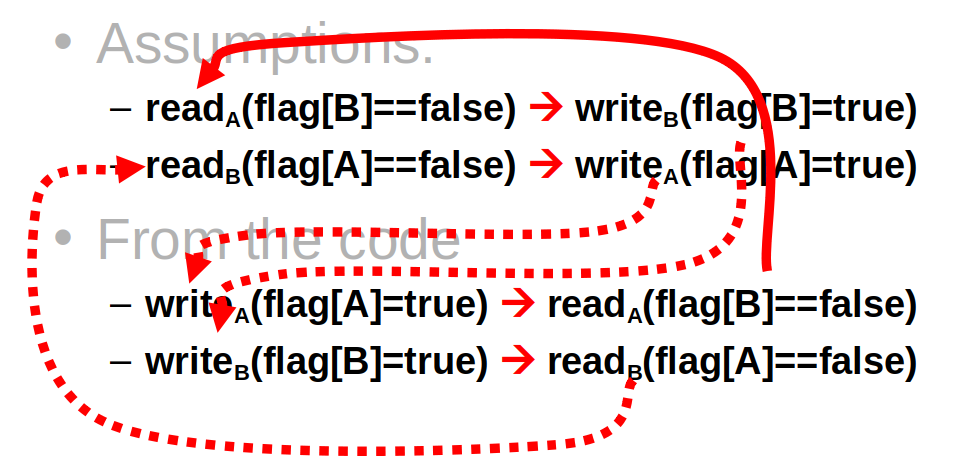
\includegraphics[width=0.8\textwidth]{./pics/lock1/combine-5.png}
\end{center}
\end{frame}

\begin{frame}[fragile,nofrmanumbering]{LockOne: mutual exclusion}
\begin{center}
  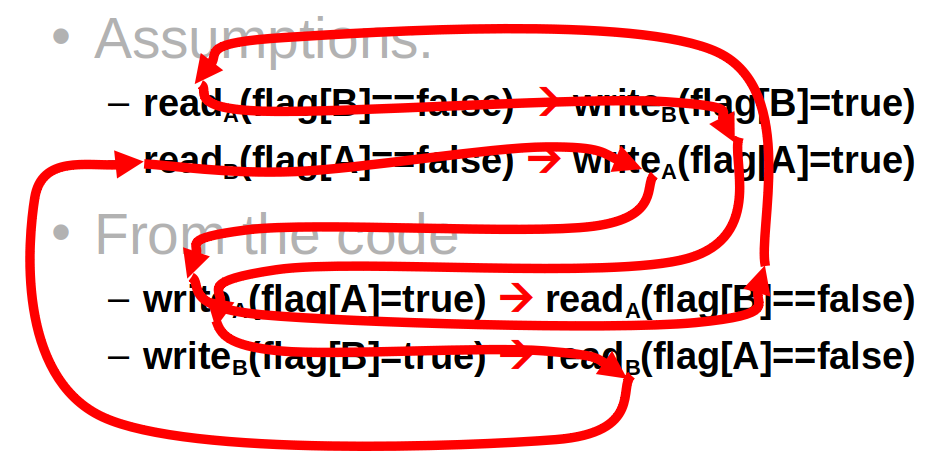
\includegraphics[width=0.8\textwidth]{./pics/lock1/combine-6.png}
\end{center}
\end{frame}

\begin{frame}[fragile,nofrmanumbering]{LockOne: mutual exclusion}
\begin{center}
  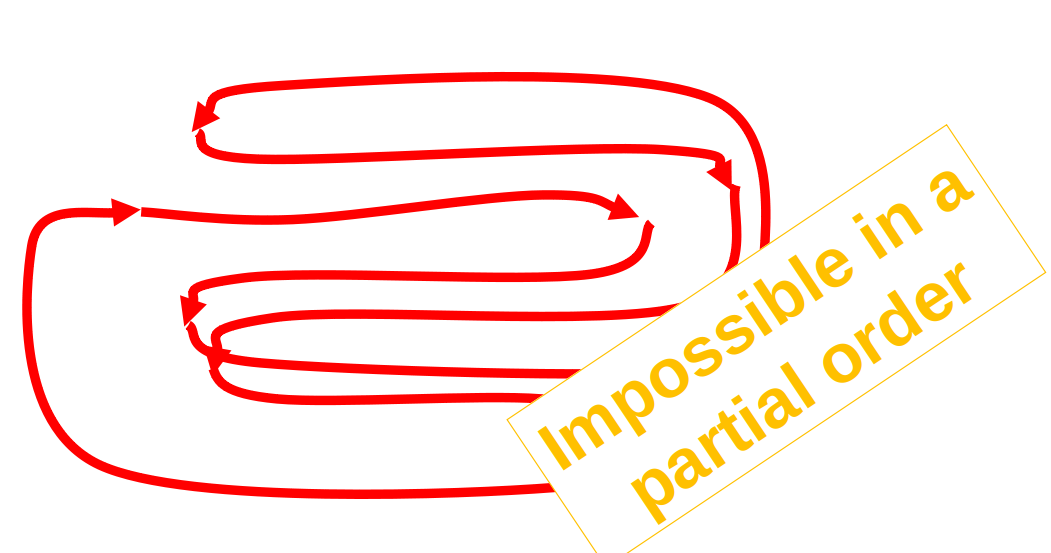
\includegraphics[width=0.8\textwidth]{./pics/lock1/combine-7.png}
\end{center}
\end{frame}



\begin{frame}[fragile]{LockOne}
\framesubtitle{Properties}

\begin{itemize}
  \item \textcolor{green}{Mutual exclusion}
  \item \textcolor{red}{Deadlock-freedom}
\end{itemize}

\pause

\begin{tabular}{p{5cm}p{5cm}}

\begin{minted}{java}
     flag[i] = true;
     while (flag[j]) {}
\end{minted}

 &  

\begin{minted}{java}
    flag[j] = true;
    while (flag[i]) {}
\end{minted}

\end{tabular}

\pause

\begin{itemize}
  \item Concurrent executions can deadlock
  \item Sequential executions OK
\end{itemize}
\end{frame}


\begin{frame}[fragile]{LockTwo}

\begin{minted}{java}
public class LockTwo implements Lock {
 private int victim;
 public void lock() {
  int i = ThreadID.get(); // 0 or 1
  victim = i;             // let the other go first
  while (victim == i) {}; // wait 
 }
 public void unlock() {}
}
\end{minted}

\pause
Satisfies Mutual Exclusion:
\begin{itemize}
  \item if thread \texttt{i} in $CS$
  \item then \texttt{victim == j}
  \item cannot be both \texttt{0} and \texttt{1}
\end{itemize}

\end{frame}


\begin{frame}[fragile]{LockTwo}

\begin{minted}{java}
public class LockTwo implements Lock {
 private int victim;
 public void lock() {
  int i = ThreadID.get(); // 0 or 1
  victim = i;             // let the other go first
  while (victim == i) {}; // wait 
 }
 public void unlock() {}
}
\end{minted}

\pause

Not deadlock free:
\begin{itemize}
  \item Sequential execution deadlocks
  \item Concurrent execution does not
\end{itemize}
\end{frame}


\begin{frame}[fragile]{LockOne and LockTwo}

LockOne, LockTwo:
\begin{itemize}
  \item \textcolor{green}{Mutual exclusion}
  \item \textcolor{red}{Deadlock-freedom}
\end{itemize}

\pause

LockOne:
\begin{itemize}
  \item Concurrent executions can deadlock
  \item Sequential executions OK
\end{itemize}

\pause

LockTwo:
\begin{itemize}
  \item Concurrent execution OK
  \item Sequential execution can deadlock
\end{itemize}

\pause

\textbf{Idea:} combine them!
\end{frame}

\begin{frame}[fragile]{Peterson’s Algorithm}

\begin{minted}{java}
class Peterson implements Lock {
  private boolean[] flag = new boolean[2];
  private int victim;
  public void lock() {
    int i = ThreadID.get(); // 0 or 1
    int j = 1 - i;
    flag[i] = true;         // I am interested
    victim  = i;            // you go first
    while (flag[j] && victim == i) {}; // wait while other interested and 
                                       // I am the victim
  }
  public void unlock() {
   flag[ThreadID.get()] = false; // I am not interested
  }
}
\end{minted}
\end{frame}

\begin{frame}[fragile]{Peterson’s Algorithm}
\framesubtitle{Mutual exclusion}

\begin{minted}{java}
public void lock() {
  flag[i] = true;         // I am interested
  victim  = i;            // you go first
  while (flag[j] && victim == i) {}; // wait while other interested and 
                                     // I am the victim
}
\end{minted}

From the code:
\begin{itemize}
  \item $write_{B}(flag[B] = true) \rightarrow write_{B}(victim = B)$
  \item $write_{A}(victim = A) \rightarrow read_{A}(flag[B]) \rightarrow read_{A}(victim)$ 
\end{itemize}

Assumption (both threads entered CS, latest to write victim is thread \texttt{A}):
\begin{itemize}
  \item $write_{B}(victim = B) \rightarrow write_{A}(victim = A)$
\end{itemize}

\end{frame}


\begin{frame}[fragile, t]{Peterson’s Algorithm}
\framesubtitle{Mutual exclusion}
\begin{itemize}
  \item $write_{B}(flag[B] = true) \rightarrow write_{B}(victim = B)$
  \item $write_{A}(victim = A) \rightarrow read_{A}(flag[B]) \rightarrow read_{A}(victim)$ 
  \item $write_{B}(victim = B) \rightarrow write_{A}(victim = A)$
\end{itemize}

\pause

Let`s swap second and third lines.

\end{frame}

\begin{frame}[fragile,t,noframenumbering]{Peterson’s Algorithm}
\framesubtitle{Mutual exclusion}
\begin{itemize}
  \item $write_{B}(flag[B] = true) \rightarrow write_{B}(victim = B)$
  \item $write_{B}(victim = B) \rightarrow write_{A}(victim = A)$
  \item $write_{A}(victim = A) \rightarrow read_{A}(flag[B]) \rightarrow read_{A}(victim)$ 
\end{itemize}

\pause

Let`s remove repeats.

\end{frame}

\begin{frame}[fragile,t,noframenumbering]{Peterson’s Algorithm}
\framesubtitle{Mutual exclusion}
\begin{itemize}
  \item $write_{B}(flag[B] = true) \rightarrow$
  \item $write_{B}(victim = B) \rightarrow$
  \item $write_{A}(victim = A) \rightarrow read_{A}(flag[B]) \rightarrow read_{A}(victim)$ 
\end{itemize}

\pause

Thread \texttt{A} read \texttt{flag[B] == true} and \texttt{victim == A} so it could not have entered the $CS$.

\pause

QED.
\end{frame}

\begin{frame}[fragile]{Peterson’s Algorithm}
\framesubtitle{Starvation freedom (implies deadlock freedom)}

\begin{minted}{java}
public void lock() {
  flag[i] = true;
  victim  = i;
  while (flag[j] && victim == i) {};                                    
}
public void unlock() {
  flag[i] = false;
}
\end{minted}

\pause

\begin{itemize}
  \item Thread \texttt{i} blocked only if \texttt{j} repeatedly re-enters so \texttt{flag[j] == true} and \texttt{victim == i}.
  \pause
  \item When thread \texttt{j} re-enters it sets \texttt{victim = j}.
  \pause
  \item So thread \texttt{i} gets in.
\end{itemize}

\end{frame}

\begin{frame}[fragile]{Summary: 2-thread mutual exclusion}

Formalize concurrent method execution:
\begin{itemize}
  \item Single timeline
  \item Totally ordered atomic events
  \item Methods represented as partially ordered intervals
  \item \textit{Precedence} is irreflexive, antisymmetric, transitive partial order
\end{itemize}

\pause

Formalize mutex properties:
\begin{itemize}
  \item Mutual exclusion
  \item Deadlock freedom
  \item Starvation freedom (implies Deadlock freedom)
\end{itemize}

\pause

Prove theorems:
\begin{itemize}
  \item Algorithm has property (\textit{suppose not ...})
  \item Algorithm lacks property (provide counterexample)
\end{itemize}

\end{frame}

\subsection{N threads}
\showTOCSub

\begin{frame}[fragile]{Filter Lock}
\framesubtitle{Idea}

There are n-1 “waiting rooms” called levels.

\begin{itemize}
  \item At each level
  \begin{itemize}
    \item At least one enters level
    \item At least one blocked if many try
  \end{itemize}
  \item Only one thread makes it through
\end{itemize}

\begin{center}
  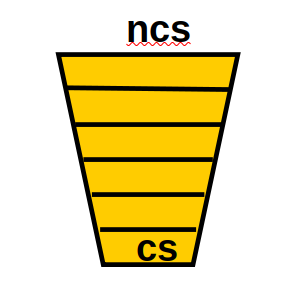
\includegraphics[width=0.2\textwidth]{./pics/filter/pyramid.png}
\end{center}

\end{frame}


\begin{frame}[fragile]{Filter Lock}
\framesubtitle{Level and victim}

\begin{minted}{java}
class Filter implements Lock {
  // level[i] for thread i
  int[] level;  
  // victim[L] for level L
  int[] victim; 
  public Filter(int n) {
    level  = new int[n];
    victim = new int[n]; 
    for (int i = 1; i < n; i++) {
      level[i] = 0;
    }
  }
}
\end{minted}

\begin{tikzpicture}[remember picture,overlay]
\node[xshift=3cm,yshift=-1.0cm] at (current page.center) {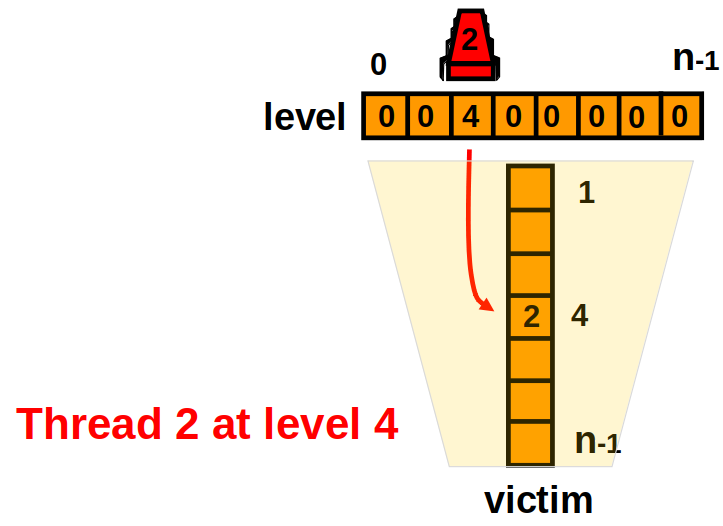
\includegraphics[width=0.5\textwidth]{./pics/filter/level_victim.png}};
\end{tikzpicture}

\end{frame}


\begin{frame}[fragile,t]{Filter Lock}
\begin{center}
  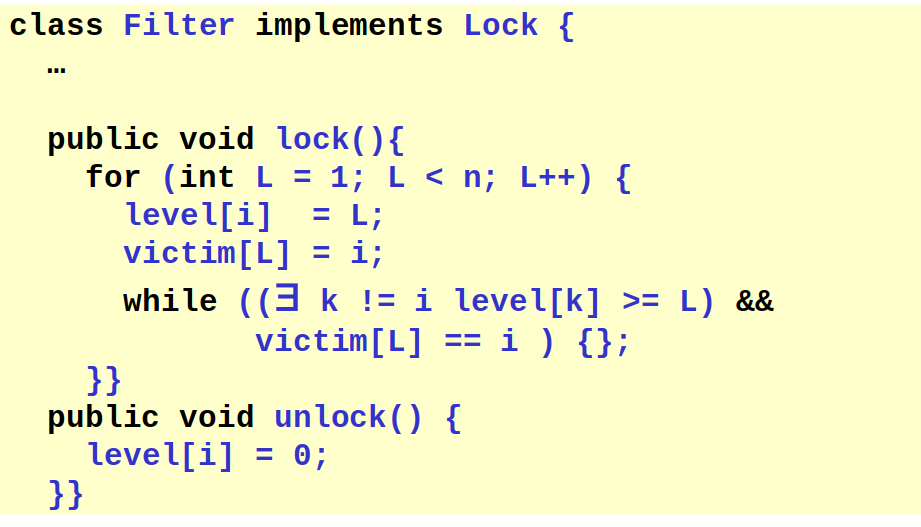
\includegraphics[width=0.6\textwidth]{./pics/filter/f1.png}
\end{center}
\end{frame}

\begin{frame}[fragile,t,noframenumbering]{Filter Lock}
\begin{center}
  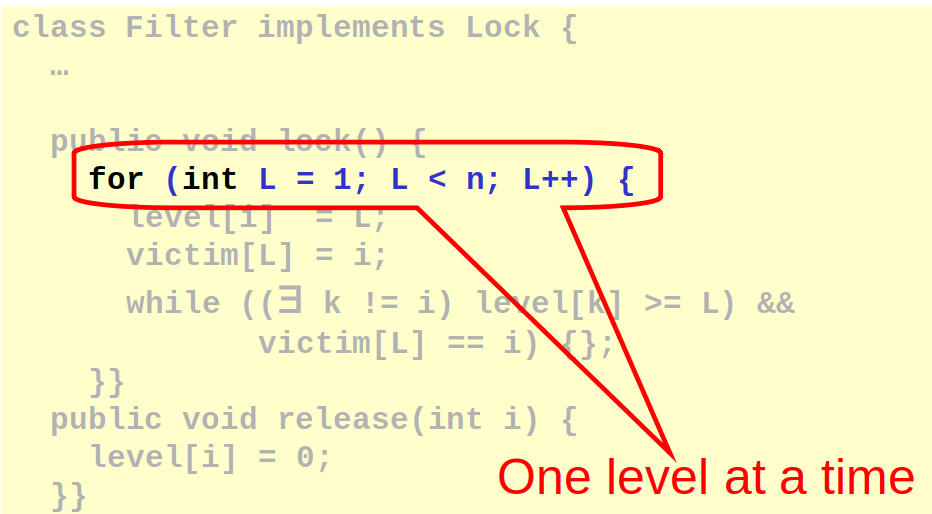
\includegraphics[width=0.6\textwidth]{./pics/filter/f2.png}
\end{center}
\end{frame}

\begin{frame}[fragile,t,noframenumbering]{Filter Lock}
\begin{center}
  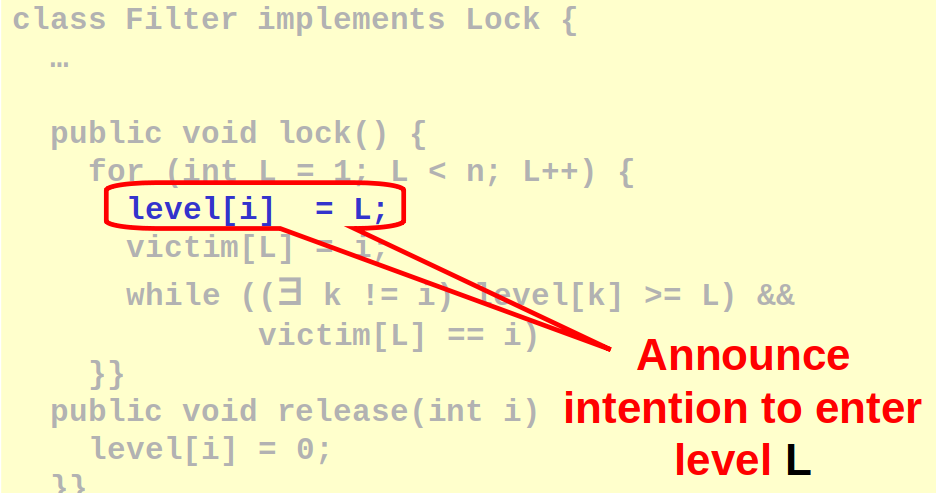
\includegraphics[width=0.6\textwidth]{./pics/filter/f3.png}
\end{center}
\end{frame}

\begin{frame}[fragile,t,noframenumbering]{Filter Lock}
\begin{center}
  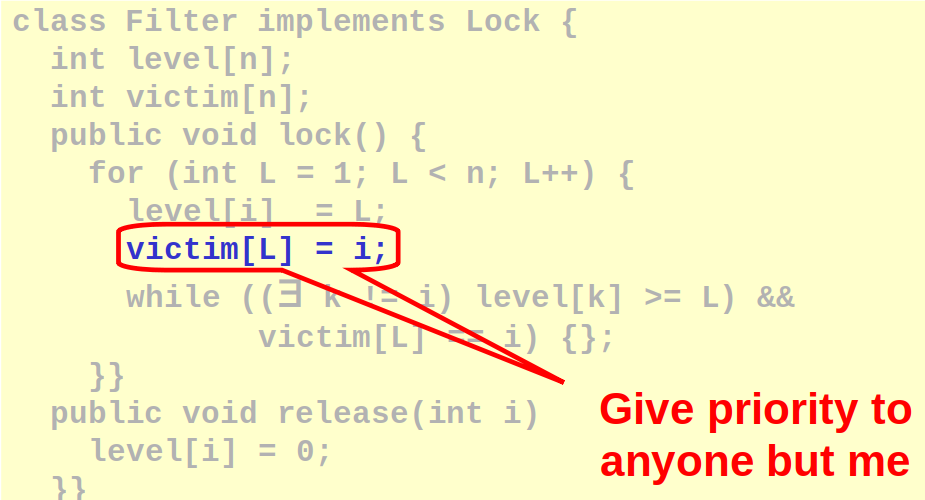
\includegraphics[width=0.6\textwidth]{./pics/filter/f4.png}
\end{center}
\end{frame}

\begin{frame}[fragile,t,noframenumbering]{Filter Lock}
\begin{center}
  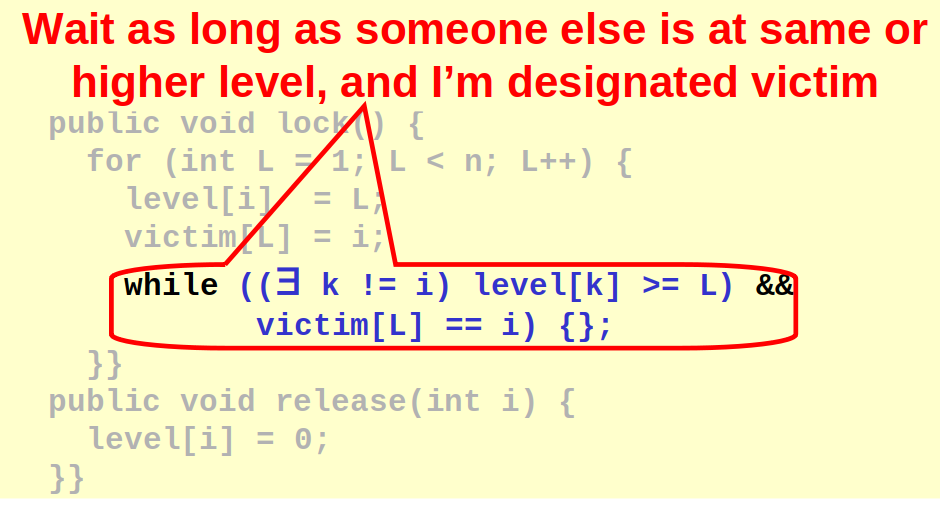
\includegraphics[width=0.6\textwidth]{./pics/filter/f5.png}
\end{center}
\end{frame}

\begin{frame}[fragile,t,noframenumbering]{Filter Lock}
\begin{center}
  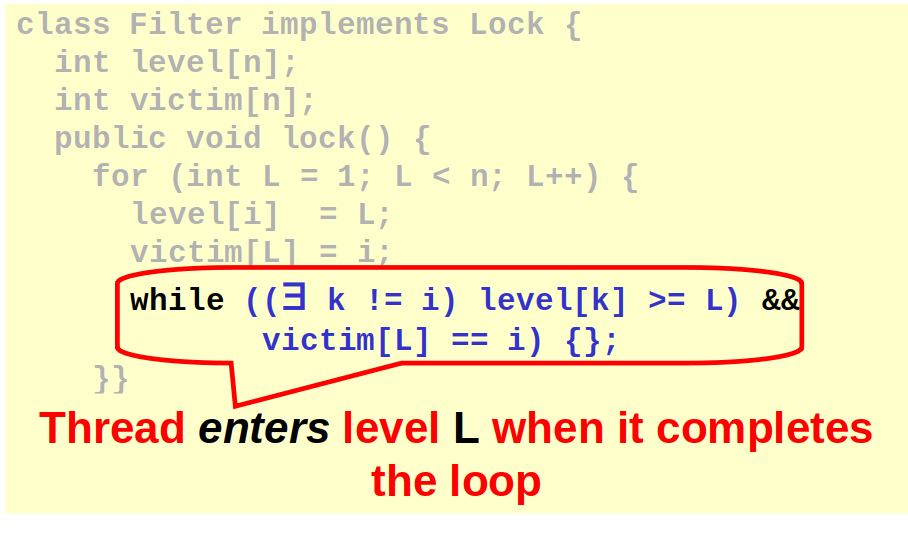
\includegraphics[width=0.6\textwidth]{./pics/filter/f6.png}
\end{center}
\end{frame}


\begin{frame}[fragile]{Filter Lock}
\framesubtitle{Proof idea}

\begin{itemize}
  \item Start at level \texttt{L = 0}
  \item At most \texttt{n - L} threads enter level \texttt{L}
  \item Mutual exclusion at level \texttt{L = n-1}
\end{itemize}

\pause

Induction Hypothesis:
\begin{itemize}
  \item No more than \texttt{n-(L-1)} at level \texttt{L-1} 
  \item Induction step: by contradiction 
  \item Assume all at level \texttt{L-1} enter level \texttt{L}
  \item Thread \texttt{A} last to write \texttt{victim[L]} 
  \item Thread \texttt{B} is any other thread at level \texttt{L}
\end{itemize}

\pause

Homework: slides 77-93 from \texttt{chapter\_02.ppt}

Homework: Section 2.4 "The Filter Lock" \ (pages 28 - 31) from "The Art of Multiprocessor Programming"

\end{frame}

\begin{frame}[fragile]{Filter Lock}
\framesubtitle{No starvation}

Filter Lock satisfies properties:
\begin{itemize}
  \item Just like Peterson Alg at any level
  \item So no one starves 
\end{itemize}

\pause
But what about fairness?

\pause
Threads can be overtaken by others 

\end{frame}


\begin{frame}[fragile]{Summary: N-thread mutual exclusion}

N-level design:
\begin{itemize}
  \item every step "filters" (prevents from progress) at least one thread
  \item reuse ideas from simpler design (2-thread Peterson`s algorithm)
\end{itemize}

\pause

We have many memory cells (\textbf{registers}\footnote<2->{Historical name}): boolean \texttt{flag[i]}, integer \texttt{victim[j]}
\begin{itemize}
  \pause
  \item \textbf{How many} registers are needed to solve N-thread mutual exclusion? 
  
  \onslide<6->{Theorem about Lower bounds, next slide}
  \pause
  \item \textbf{What} are those registers? How to describe them formally? 
  
  \onslide<7->{Concurrent objects chapter, later today}
  \pause
  \item Is there any \textbf{alternative} to registers and how to use it to implement mutual exclusion? 
  
  \onslide<8->{Lecture~\atomicsNum}
\end{itemize}

\end{frame}

\subsection{Lower bounds on the Number of Locations}
\showTOCSub

\begin{frame}{Mutual exclusion for N threads requires read-write of at least N locations}

Optional homework:
\begin{quote}
  Theorem 2.8.1. Any \texttt{Lock} algorithm that, by reading and writing memory, solves deadlock-free mutual exclusion for three threads must
  use at least three distinct memory locations.
\end{quote}

Key insights:
\begin{itemize}
  \item Covering state
\end{itemize}

Generalized theorem: $N$-thread deadlock-free mutual exclusion requires $N$ distinct locations.

\end{frame}


\begin{frame}[fragile]{Mutual exclusion: you know so far}

Mutual exclusion could be solved:
\begin{itemize}
  \item For \texttt{N} concurrent threads
  \item Using \texttt{N} boolean and \texttt{N} integer registers
  \item Provides starvation-freedom
\end{itemize}

\pause

Mutual exclusion could not be solved:
\begin{itemize}
  \item Using less than \texttt{N} registers
\end{itemize}

\pause

Few questions remain:
\begin{itemize}
  \pause
  \item How much time will thread wait until success? \texttt{FilterLock} does not guarantee fairness

  \pause
  \item Could we "improve" \ registers with some additional operations to speed-up the algorithm?

  \pause
  \item What if threads are created and deleted dynamically?

\end{itemize}
\end{frame}

\subsection{Optional: fairness}
\showTOCSub

\begin{frame}[fragile]{Formalizing fairness}

Optional homework: slides 95-99 from \texttt{chapter\_02.ppt}

Optional homework: Section 2.5 "Fairness" \ (page 31)

Key insights: 
\begin{itemize}
  \item \textit{doorway} section
  \item \textit{waiting} section
  \item \textiti{first-come-first-served} ($D_{A}^{j} \rightarrow D_{B}^{k}$ then $CS_{A}^{j} \rightarrow CS_{B}^{k}$)
\end{itemize}

\end{frame}

\begin{frame}[fragile]{Bakery algorithm}

Optional homework: slides 99-118 from \texttt{chapter\_02.ppt}

Optional homework: Section 2.6 "Lamport`s Bakery Algorithm" \ (pages 31 - 33)

Key insights: 
\begin{itemize}
  \item monotonically growing labels for operations
  \item proving fairness
\end{itemize}

\end{frame}

\subsection{Mutual exclusion beyond read-write memory cells}
\showTOCSub

\begin{frame}[fragile]{Mutual exclusion using read/write locations}

\begin{itemize}
  \item Correct, starvation-free algorithm exists (filter lock)
  \item Correct, starvation-free and fair algorithm exists (bakery algorithm)
  \item Any correct algorithm will require at least $N$ registers with read and write operations
\end{itemize}

\pause
We could classify registers by allowed concurrency:
\begin{itemize}
  \item Single Reader Single Writer (SRSW)
  \item Multiple Reader Single Writer (MRSW)
  \item Multiple Reader Multiple Writer (MRMW)
\end{itemize}

\pause
We could classify registers by capacity:
\begin{itemize}
  \item Boolean register ($true/false$), Integer register ($0, 1, ..., 2^N$)
\end{itemize}

\pause
We could classify registers by supported operations:
\begin{itemize}
  \item Read-only, Write-once, Monotonically increasing, Arbitrary update
  \pause
  \item Atomic read-modify-write operations
\end{itemize}

\pause

Before diving into classifications (Lecture~\foundationsPlusNum, Lecture~\atomicsNum), let`s study few more mathematical instruments.

\end{frame}


\begin{frame}[fragile]{Homework: before final exam}

When you finish all lectures of second block, you will know many advanced concepts:
\begin{itemize}
  \item Concurrent object consistency definitions
  \item Register constructions
  \item Atomic snapshots
  \item Consensus number
\end{itemize}

Revise all the correctness proofs from this lecture and be ready to answer some tricky questions:
\begin{itemize}
  \item In order to prove correctness of Peterson`s algorithm, should we use MRSW or MRMW register?
  \item In order to prove correctness of mutual exclusion primitives, should we require all registers to be linearizable or weaker guarantees will fit?
  \item Could you adapt \texttt{FilterLock} to allow dynamic thread creation and deletion?
\end{itemize}

\end{frame}


%%%%%%%%%%%%%%%%%%%%%%%%%%%%
\section{Concurrent objects}
\showTOC

\subsection{Sequential and concurrent objects}

\begin{frame}{Motivation}

We need to formalize
\begin{itemize}
  \item Safety (correctness)
  \item Liveness (progress)
\end{itemize}

\pause

for concurrent data structures and concurrent algorithms.

\pause
\begin{itemize}
  \item How to define safety and liveness "universally"?
  \item How to reason about whole programs / software components in isolation?
  \item How to compose modules and correctness proofs?
  \item Are there "better" \ or "simpler" \ approaches?
\end{itemize}
\end{frame}



\begin{frame}{Concurrent objects}

Goals:
\begin{itemize}
  \item \textbf{Describe} object
  \item \textbf{Implement} object
  \item \textbf{Check} for errors
\end{itemize}

\pause
\textbf{Check} that \textbf{implementation} conforms to \textbf{specification}.

\pause
Let's focus on descriptions: \pause
\begin{itemize}
  \item when implementation is \textbf{correct}
  \item the conditions under which it guarantees \textbf{progress}
\end{itemize}

\end{frame}


\begin{frame}{Sequential objects and specifications}

Sequential object:
\begin{itemize}
  \item State
  \begin{itemize}
    \item Set of fields
  \end{itemize}
  \item Methods
  \begin{itemize}
    \item The only way to change state
  \end{itemize}
\end{itemize}

\pause 

Sequential specification:
\begin{itemize}
  \item If (\textbf{precondition}) 
  \begin{itemize}
    \item the object is in such-and-such a state
    \item before you call the method
  \end{itemize}

  \item Then (\textbf{postcondition})
  \begin{itemize}
    \item the method will return a particular value
    \item or throw a particular exception
  \end{itemize}

  \item and (\textbf{postcondition})
  \begin{itemize}
    \item the object will be in some other state
    \item when the method returns
  \end{itemize}
\end{itemize}
\end{frame}

\begin{frame}{Sequential specifications}

\begin{itemize}
  \item Interactions among methods captured by side-effects on object state
  \begin{itemize}
    \item State meaningful between method calls    
  \end{itemize}

  \item Documentation size linear in number of methods
  \begin{itemize}
    \item Each method described in isolation
  \end{itemize}

  \item Can add new methods
  \begin{itemize}
    \item Without changing descriptions of old methods
  \end{itemize}
\end{itemize}

\end{frame}


\begin{frame}{Sequential vs concurrent}

Key difference (concurrency):
\begin{itemize}
    \item Method call is not an event
    \item Method call is an interval
\end{itemize}

\pause
Implications:
\pause
\begin{itemize}
  \item method calls could overlap, object might never be between method calls
  \begin{itemize}
    \pause
    \item in sequential specification we need to only define object state between method calls
  \end{itemize}
  \pause

  \item must characterize all possible interactions with concurrent calls 
  \begin{itemize}
    \pause
    \item in sequential specification we described methods in isolation
  \end{itemize}

  \pause

  \item everything can potentially interact with everything else
  \begin{itemize}
    \pause
    \item in sequential specification we could add new methods without affecting older methods
  \end{itemize}
\end{itemize}

\pause
\begin{tikzpicture}[remember picture,overlay]
\node[xshift=2cm,yshift=-2.0cm] at (current page.center) {
\includegraphics[width=0.5\textwidth]{./pics/fry-pain-head.png}};
\end{tikzpicture}

\end{frame}


\subsection{Intuition behind consistency definitions}
\showTOCSub

\begin{frame}{Consistency}

What does it \textbf{mean} for a \textit{concurrent} object to be correct?
\begin{itemize}
  \item What is a concurrent FIFO queue?
  \pause
  \item FIFO means strict temporal order
  \item Concurrent means ambiguous temporal order
\end{itemize}
\end{frame}

\begin{frame}[fragile, noframenumbering]{Consistency}
\begin{center}
  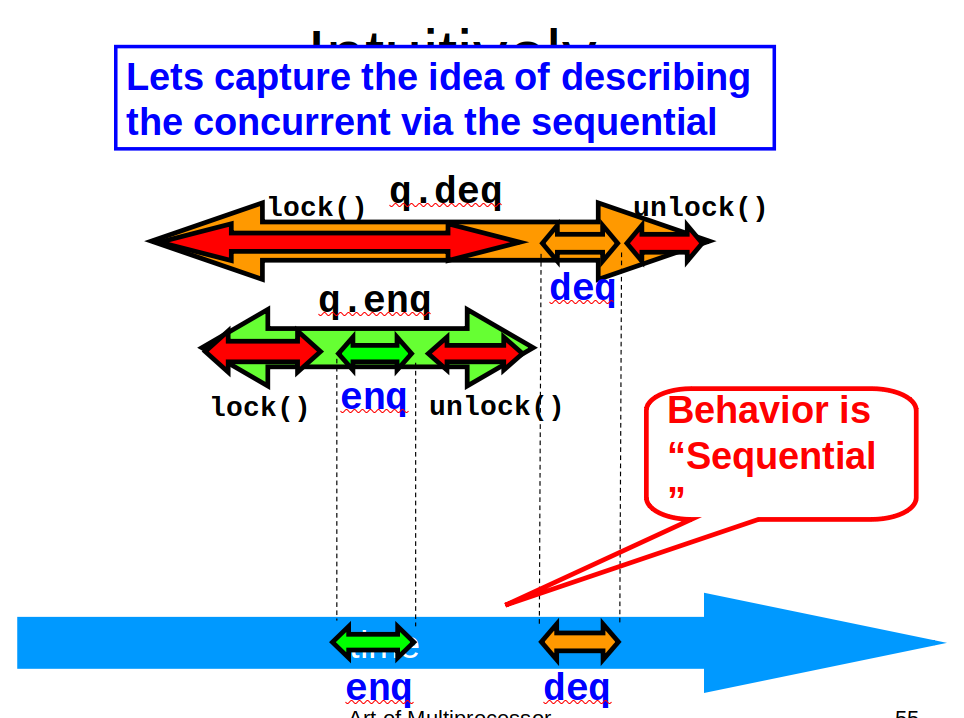
\includegraphics[width=0.5\textwidth]{./pics/conc-obj/seq-idea.png}
\end{center}
\end{frame}

\begin{frame}{Linearizability}

Each method should
\begin{itemize}
  \item “take effect”
  \item instantaneously
  \item between invocation and response events
\end{itemize}

\pause

Object is correct if this “sequential” behavior is correct

\pause
Any such concurrent object is \textbf{Linearizable}

\pause
Sounds like a property of an execution ...

\pause

A \textbf{linearizable object}: one all of whose possible executions are linearizable

\end{frame}


\begin{frame}[fragile]{Examples}
\begin{center} 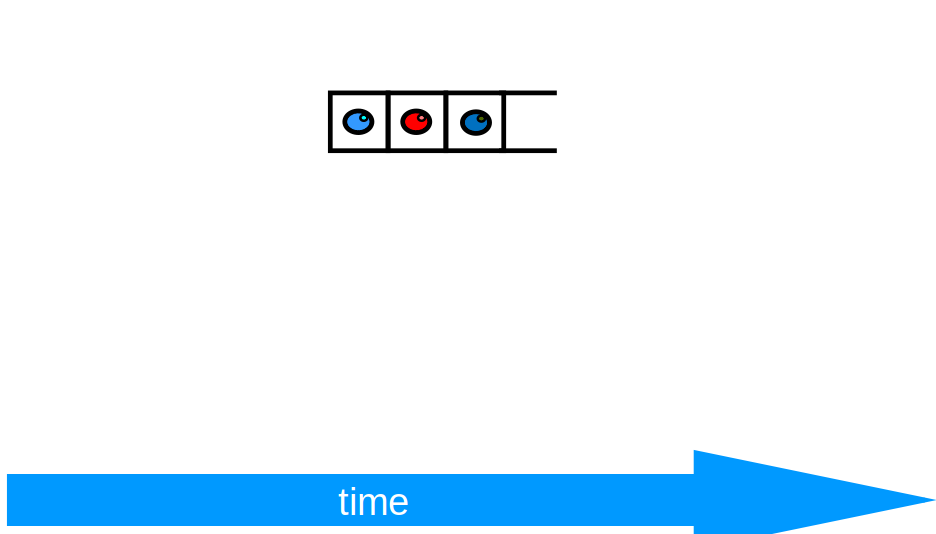
\includegraphics[width=0.7\textwidth]{./pics/linear/58.png} \end{center}
\end{frame}

\begin{frame}[fragile,noframenumbering]{Examples}
\begin{center} 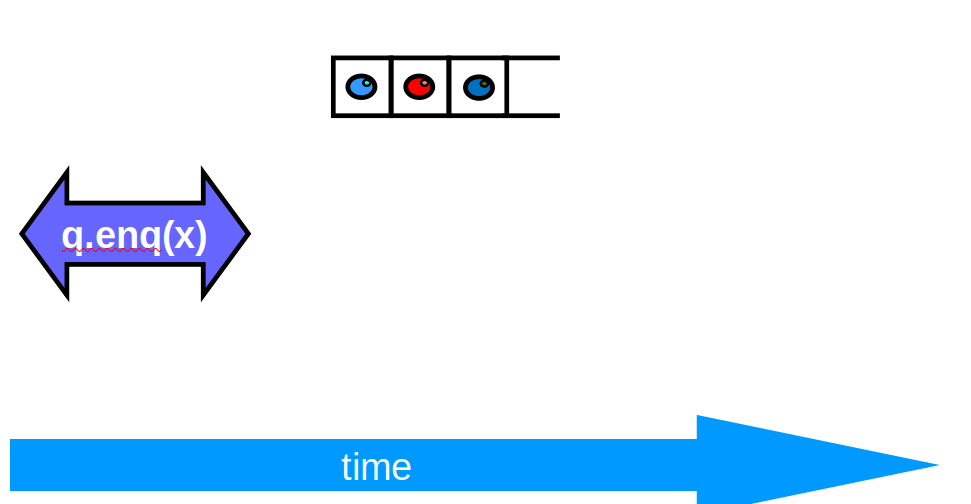
\includegraphics[width=0.7\textwidth]{./pics/linear/59.png} \end{center}
\end{frame}

\begin{frame}[fragile,noframenumbering]{Examples}
\begin{center} 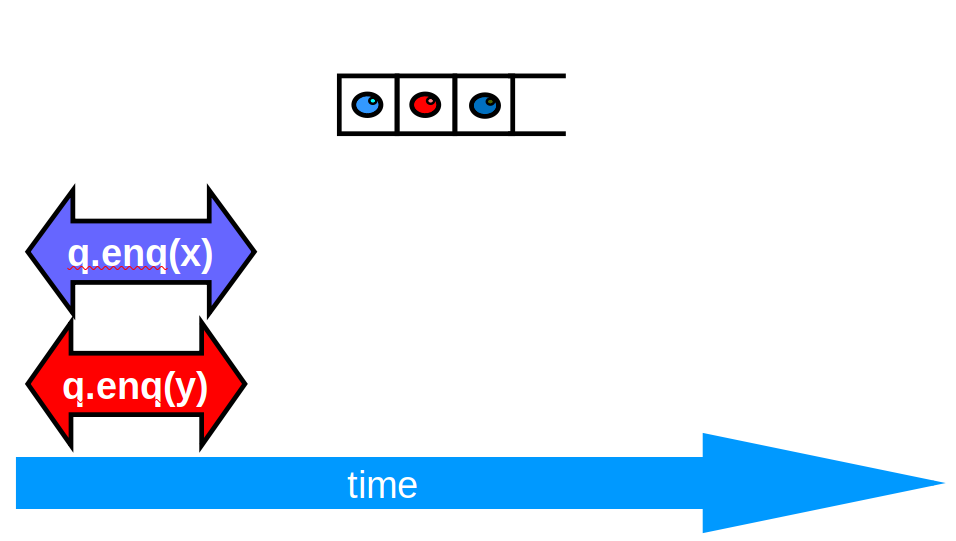
\includegraphics[width=0.7\textwidth]{./pics/linear/60.png} \end{center}
\end{frame}

\begin{frame}[fragile,noframenumbering]{Examples}
\begin{center} 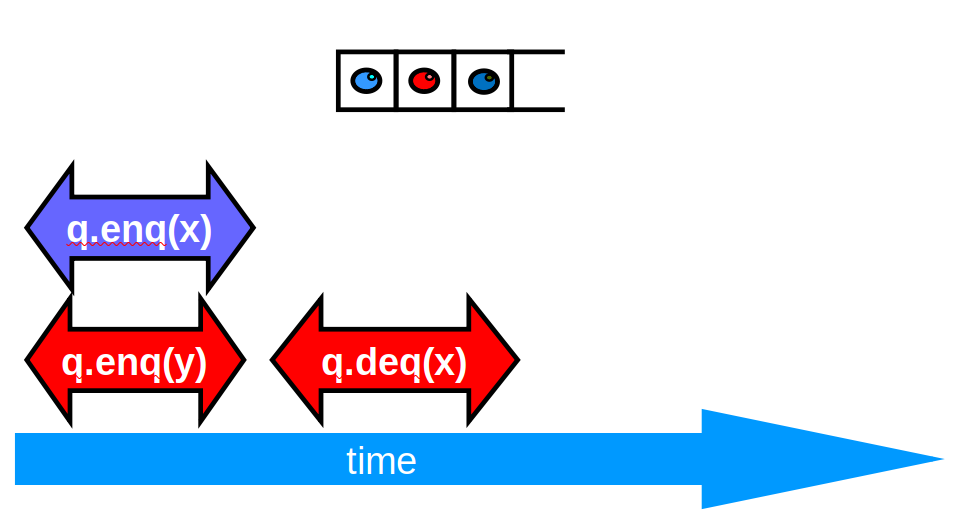
\includegraphics[width=0.7\textwidth]{./pics/linear/61.png} \end{center}
\end{frame}

\begin{frame}[fragile,noframenumbering]{Examples}
\begin{center} 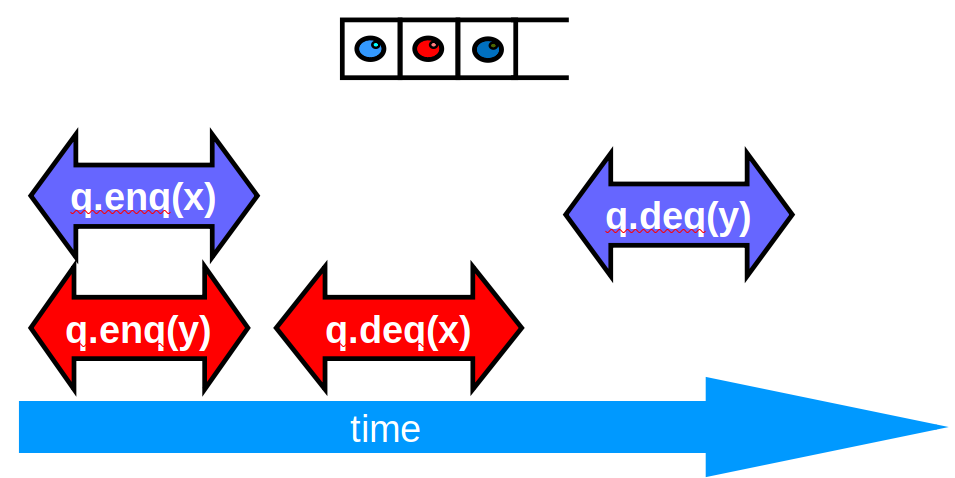
\includegraphics[width=0.7\textwidth]{./pics/linear/62.png} \end{center}
\end{frame}

\begin{frame}[fragile,noframenumbering]{Examples}
\begin{center} 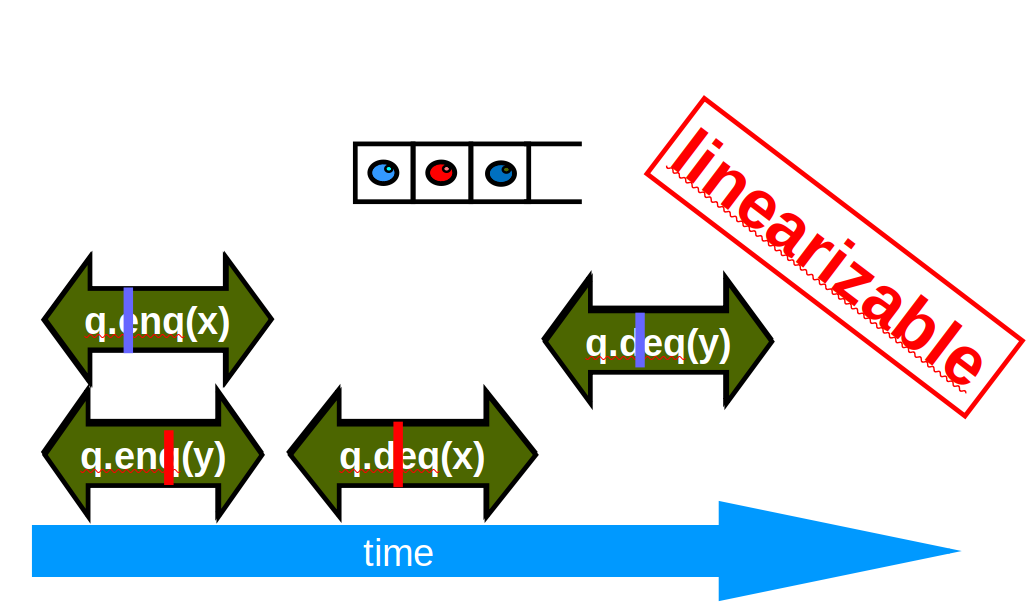
\includegraphics[width=0.7\textwidth]{./pics/linear/63.png} \end{center}
\end{frame}



\begin{frame}[fragile,noframenumbering]{Examples}
\begin{center} 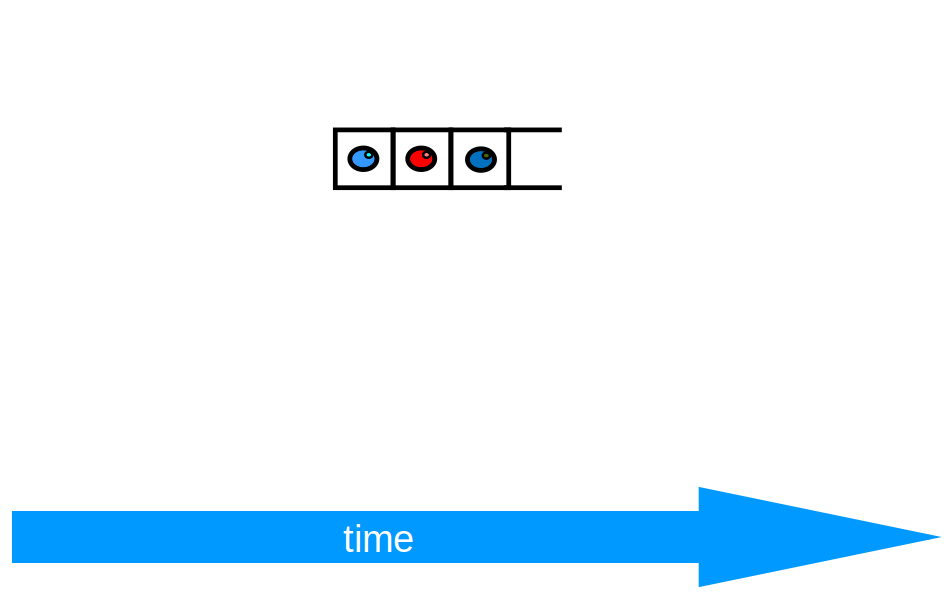
\includegraphics[width=0.7\textwidth]{./pics/linear/65.png} \end{center}
\end{frame}

\begin{frame}[fragile,noframenumbering]{Examples}
\begin{center} 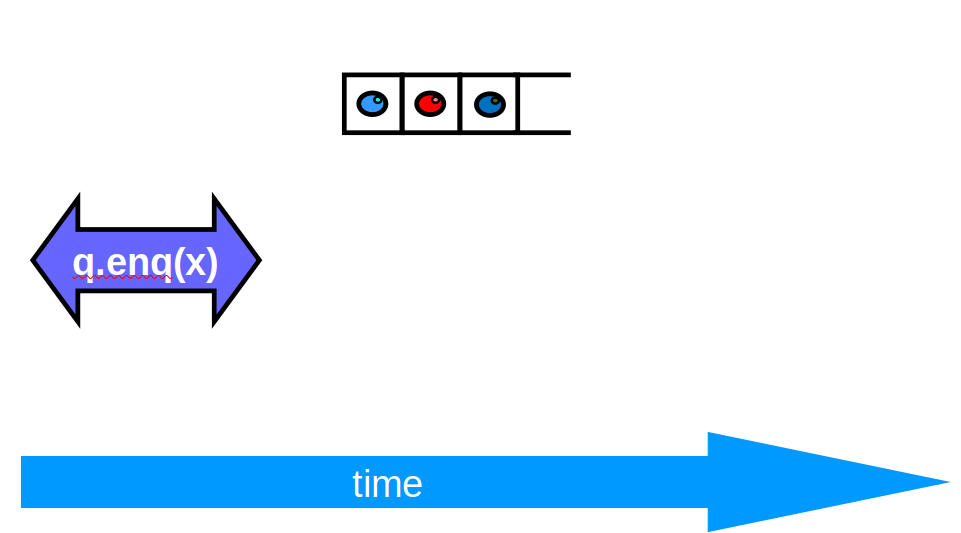
\includegraphics[width=0.7\textwidth]{./pics/linear/66.png} \end{center}
\end{frame}

\begin{frame}[fragile,noframenumbering]{Examples}
\begin{center} 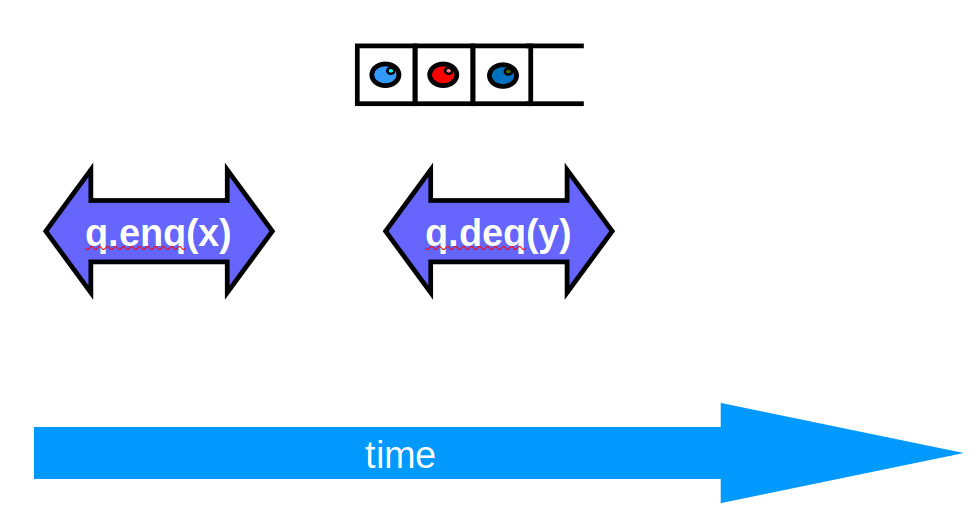
\includegraphics[width=0.7\textwidth]{./pics/linear/67.png} \end{center}
\end{frame}

\begin{frame}[fragile,noframenumbering]{Examples}
\begin{center} 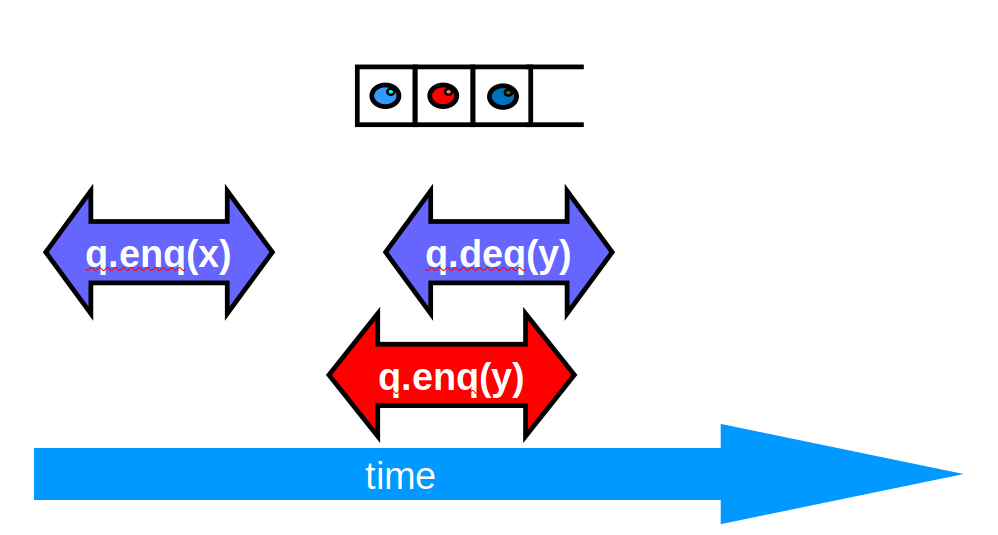
\includegraphics[width=0.7\textwidth]{./pics/linear/68.png} \end{center}
\end{frame}

\begin{frame}[fragile,noframenumbering]{Examples}
\begin{center} 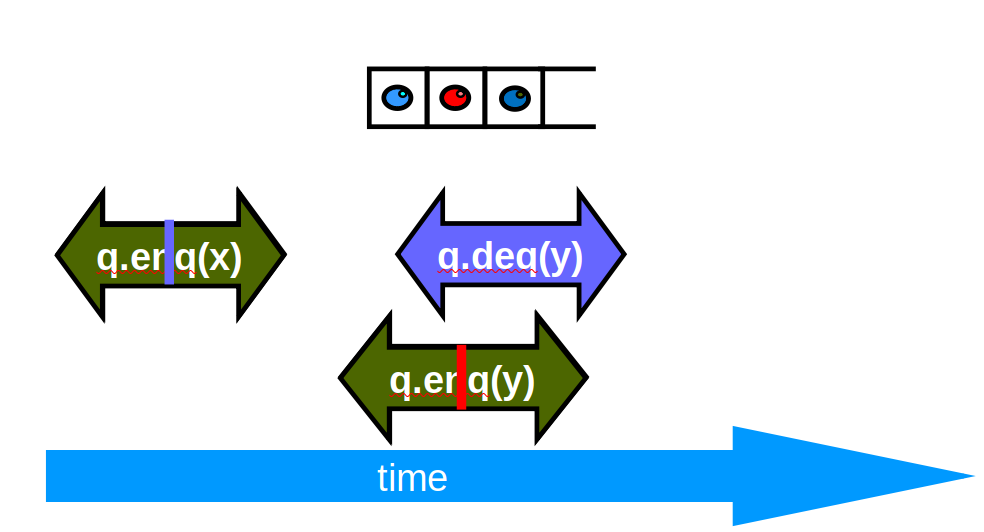
\includegraphics[width=0.7\textwidth]{./pics/linear/69.png} \end{center}
\end{frame}

\begin{frame}[fragile,noframenumbering]{Examples}
\begin{center} 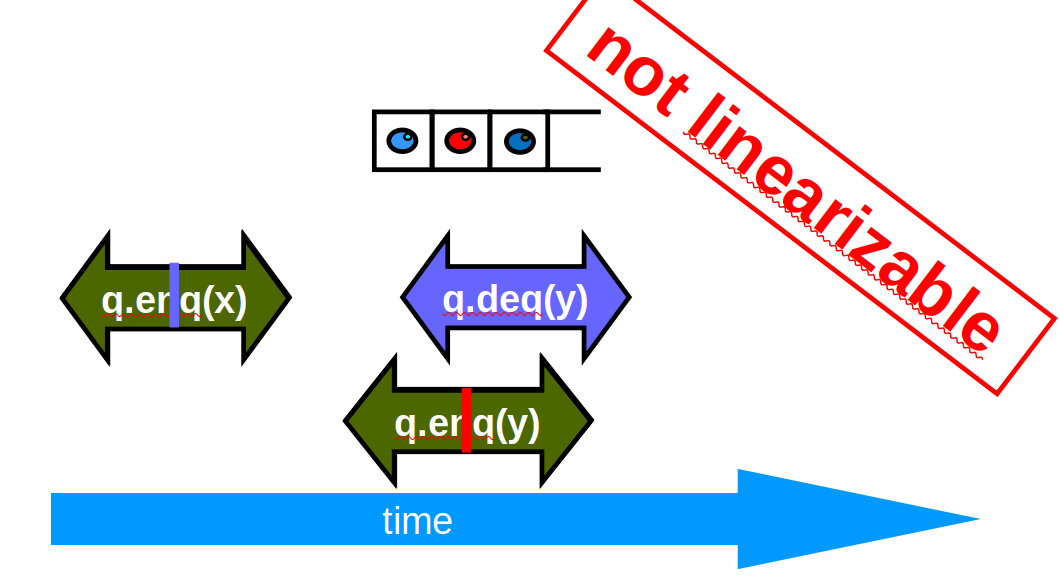
\includegraphics[width=0.7\textwidth]{./pics/linear/70.png} \end{center}
\end{frame}

\begin{frame}[fragile,noframenumbering]{Examples}
\begin{center} 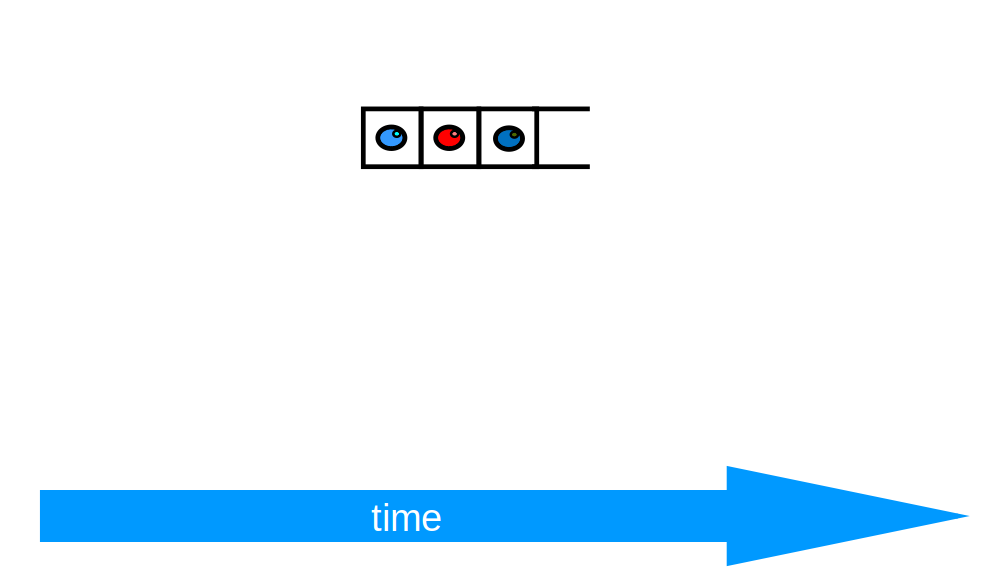
\includegraphics[width=0.7\textwidth]{./pics/linear/71.png} \end{center}
\end{frame}

\begin{frame}[fragile,noframenumbering]{Examples}
\begin{center} 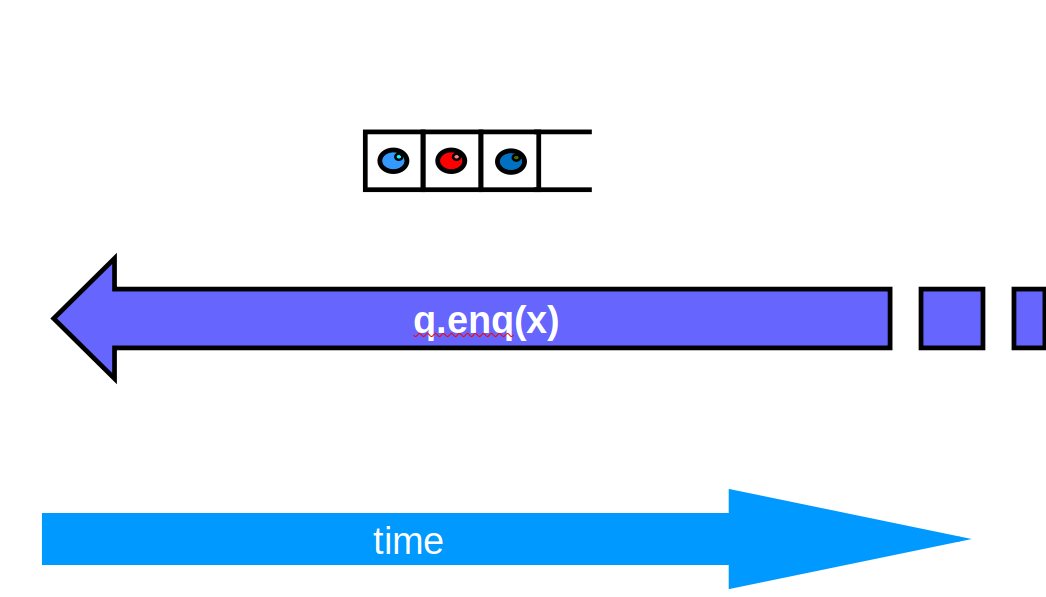
\includegraphics[width=0.7\textwidth]{./pics/linear/72.png} \end{center}
\end{frame}

\begin{frame}[fragile,noframenumbering]{Examples}
\begin{center} 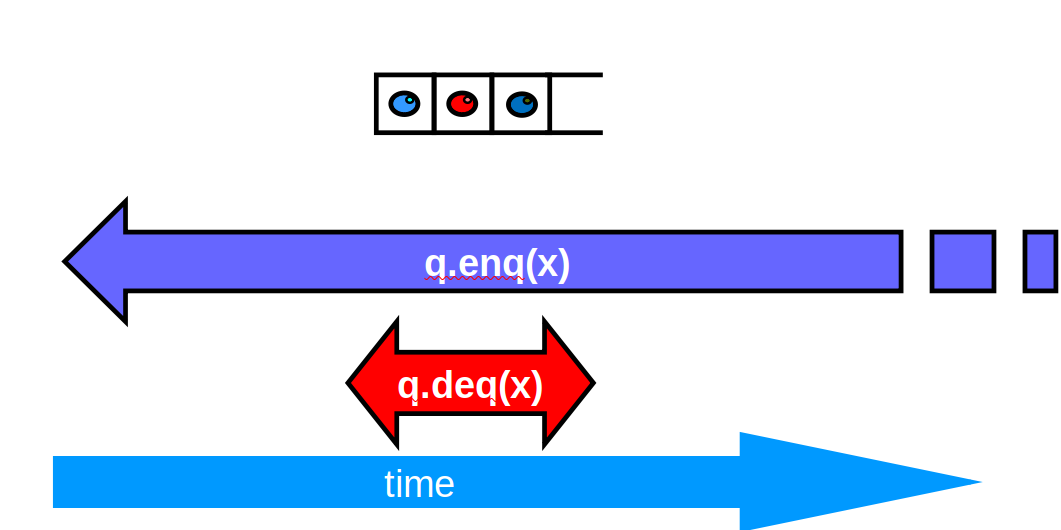
\includegraphics[width=0.7\textwidth]{./pics/linear/73.png} \end{center}
\end{frame}

\begin{frame}[fragile,noframenumbering]{Examples}
\begin{center} 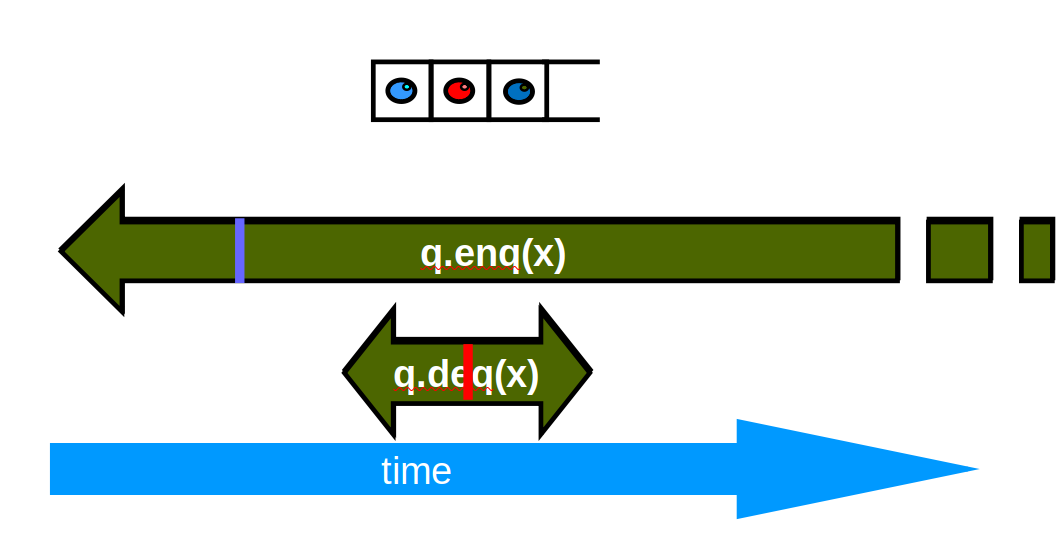
\includegraphics[width=0.7\textwidth]{./pics/linear/74.png} \end{center}
\end{frame}

\begin{frame}[fragile,noframenumbering]{Examples}
\begin{center} 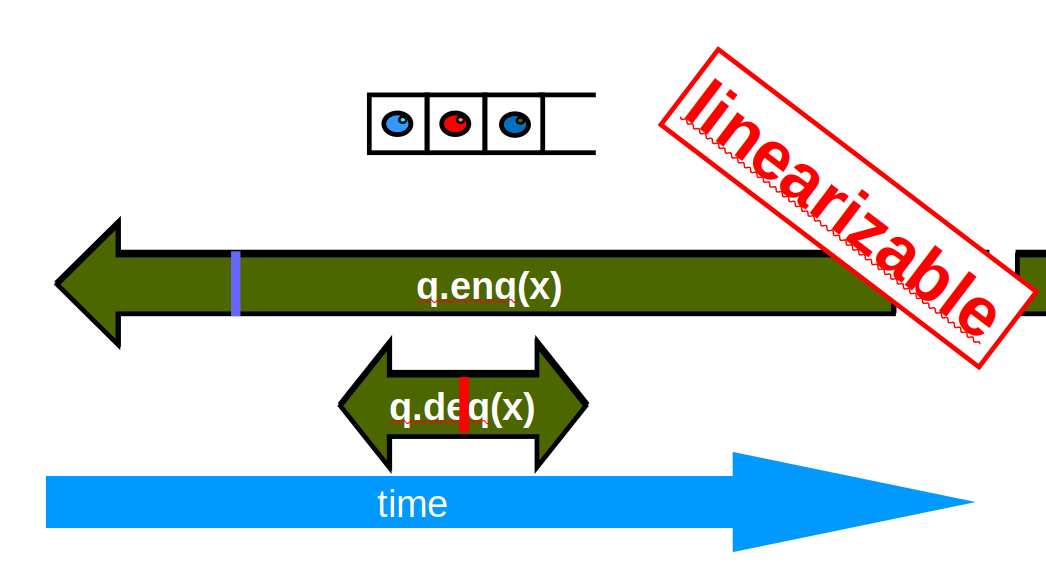
\includegraphics[width=0.7\textwidth]{./pics/linear/75.png} \end{center}
\end{frame}

\begin{frame}[fragile,noframenumbering]{Examples}
\begin{center} 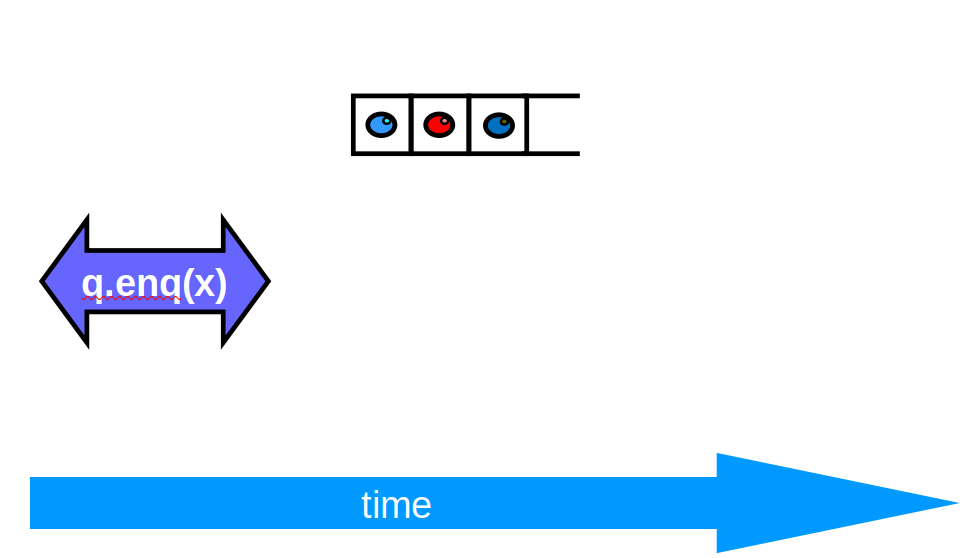
\includegraphics[width=0.7\textwidth]{./pics/linear/76.png} \end{center}
\end{frame}

\begin{frame}[fragile,noframenumbering]{Examples}
\begin{center} 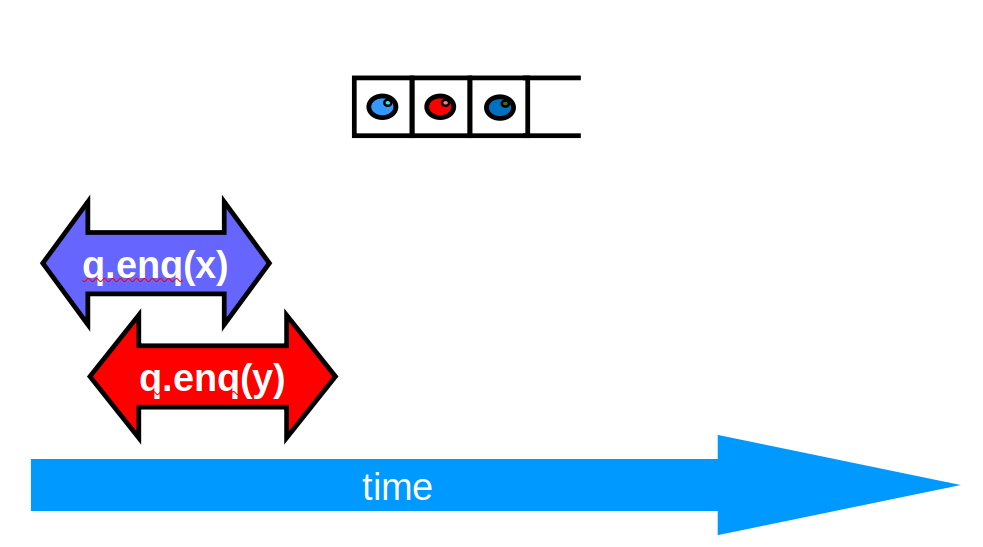
\includegraphics[width=0.7\textwidth]{./pics/linear/77.png} \end{center}
\end{frame}

\begin{frame}[fragile,noframenumbering]{Examples}
\begin{center} 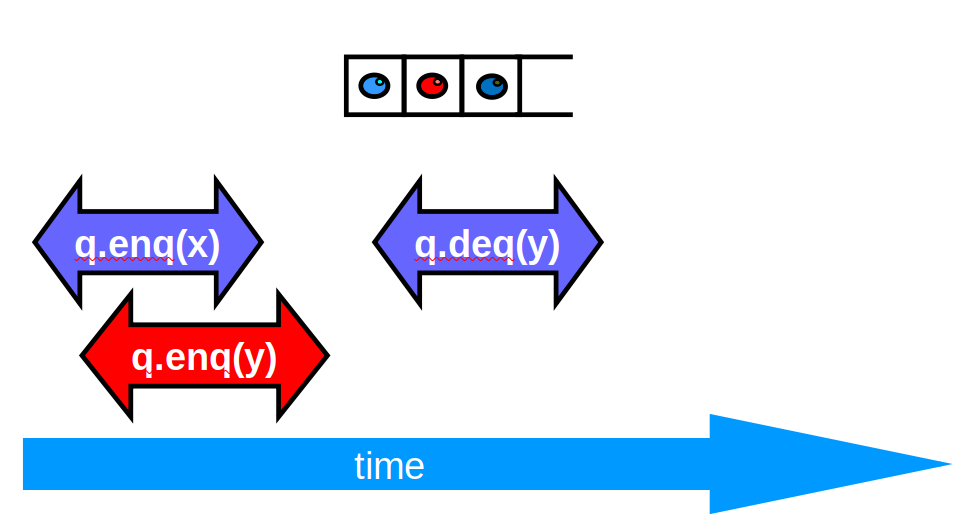
\includegraphics[width=0.7\textwidth]{./pics/linear/78.png} \end{center}
\end{frame}

\begin{frame}[fragile,noframenumbering]{Examples}
\begin{center} 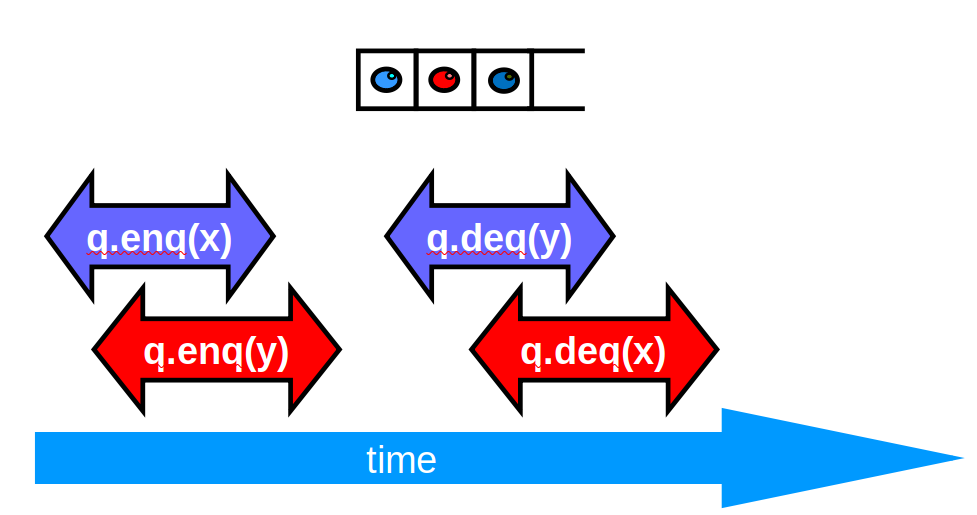
\includegraphics[width=0.7\textwidth]{./pics/linear/79.png} \end{center}
\end{frame}

\begin{frame}[fragile,noframenumbering]{Examples}
\begin{center} 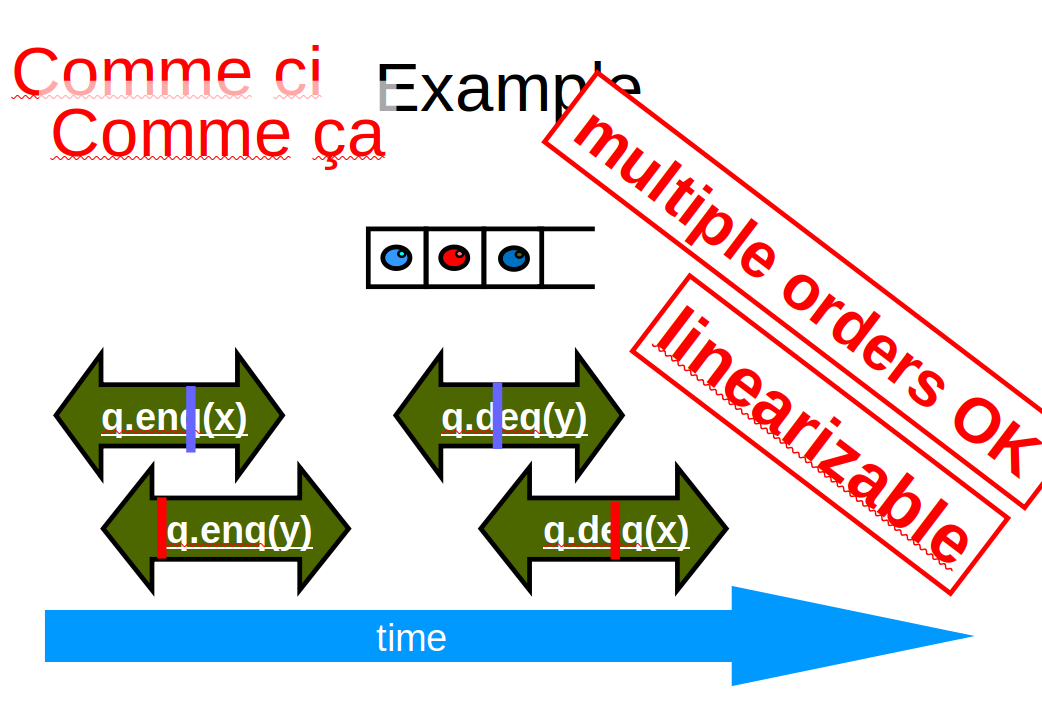
\includegraphics[width=0.7\textwidth]{./pics/linear/80.png} \end{center}
\end{frame}

\begin{frame}[fragile,noframenumbering]{Examples}
\begin{center} 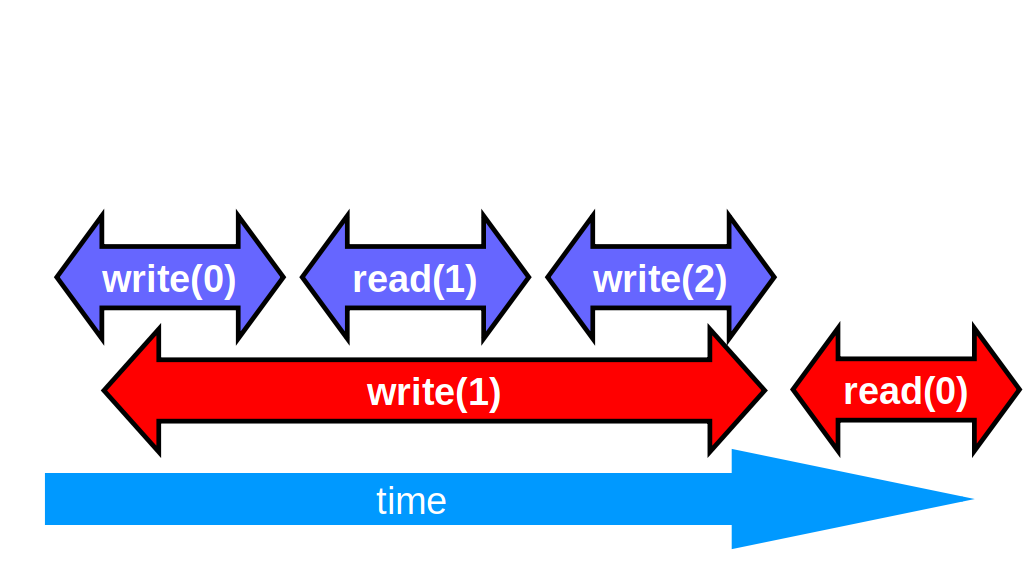
\includegraphics[width=0.7\textwidth]{./pics/linear/81.png} \end{center}
\end{frame}

\begin{frame}[fragile,noframenumbering]{Examples}
\begin{center} 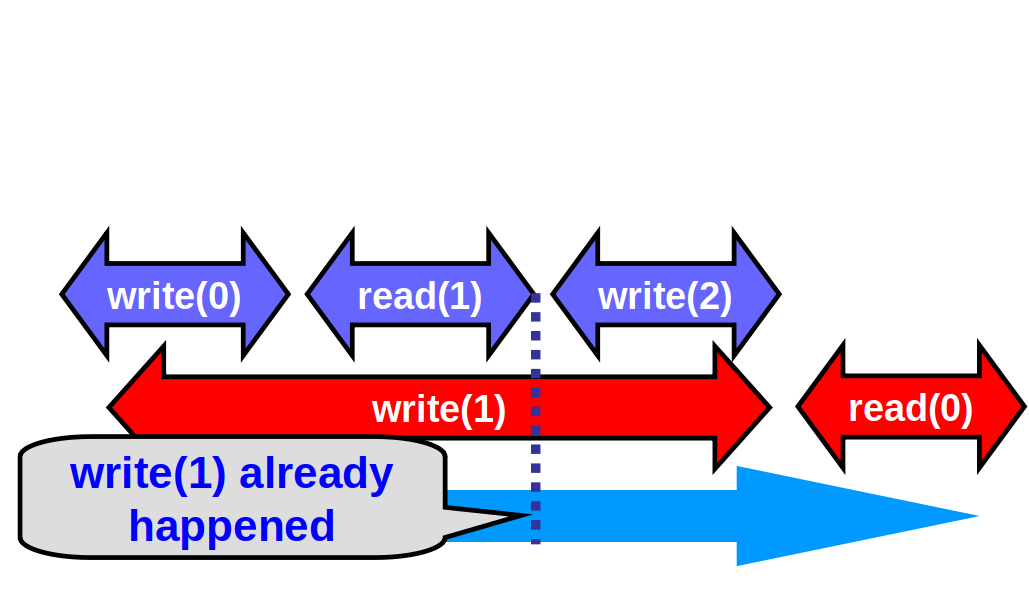
\includegraphics[width=0.7\textwidth]{./pics/linear/82.png} \end{center}
\end{frame}

\begin{frame}[fragile,noframenumbering]{Examples}
\begin{center} \includegraphics[width=0.7\textwidth]{./pics/linear/83.png} \end{center}
\end{frame}

\begin{frame}[fragile,noframenumbering]{Examples}
\begin{center} \includegraphics[width=0.7\textwidth]{./pics/linear/84.png} \end{center}
\end{frame}

\begin{frame}[fragile,noframenumbering]{Examples}
\begin{center} \includegraphics[width=0.7\textwidth]{./pics/linear/85.png} \end{center}
\end{frame}

\begin{frame}[fragile,noframenumbering]{Examples}
\begin{center} \includegraphics[width=0.7\textwidth]{./pics/linear/86.png} \end{center}
\end{frame}

\begin{frame}[fragile,noframenumbering]{Examples}
\begin{center} \includegraphics[width=0.7\textwidth]{./pics/linear/87.png} \end{center}
\end{frame}

\begin{frame}[fragile,noframenumbering]{Examples}
\begin{center} \includegraphics[width=0.7\textwidth]{./pics/linear/88.png} \end{center}
\end{frame}

\begin{frame}[fragile,noframenumbering]{Examples}
\begin{center} \includegraphics[width=0.7\textwidth]{./pics/linear/89.png} \end{center}
\end{frame}

\begin{frame}[fragile,noframenumbering]{Examples}
\begin{center} \includegraphics[width=0.7\textwidth]{./pics/linear/90.png} \end{center}
\end{frame}


\begin{frame}{Linearizability: summary}

Each method should
\begin{itemize}
  \item “take effect”
  \item instantaneously
  \item between invocation and response events
\end{itemize}

Linearization point: when method "commit changes to object state"
\begin{itemize}
  \item Could be different code points for different executions!
\end{itemize}

Linearizability
\begin{itemize}
 \item requires to analyze executions, not just methods
 \item compositional -- result of composing linearizable objects is linearizable\footnote{Optional homework: Theorem 3.6.1 in "The Art of Multiprocessor Programming"}
\end{itemize}

\end{frame}


\begin{frame}[fragile]{Linearizability is not the only one}

There exists:
\begin{itemize}
  \pause
  \item Sequential consistency
  \begin{itemize}
    \item Provides other guarantees, harder to reason (no linearization points)
    \item \textbf{Not} compositional
    \item Hardware designers love to use weaker variations of it (Lecture~\cacheCoherencyNum \ will be hard)    
  \end{itemize}

  \pause
  \item Quiescent consistency
  \begin{itemize}
    \item One of the weakest (yet understandable) consistencies
    \item Compositional
    \item Complicated performance-oriented concurrent data structures may use it to formalize possible and impossible results
  \end{itemize}
\end{itemize}

\pause

Linearizability is useful yet could be not applicable (by design\footnote<4->{\tiny{RCU: advantages and disadvantages \url{https://en.wikipedia.org/wiki/Read-copy-update}}} or by implementation\footnote<4->{\tiny{ConcurrentLinkedDeque is non-linearizable \url{https://bugs.openjdk.org/browse/JDK-8256833}}})

\end{frame}


\begin{frame}[fragile]{Intuition behind consistency definitions: takeaways}

\begin{itemize}
  \item \textbf{Describe} object first, then implement and test it
  \item Sequential specifications totally rock
  \begin{itemize}
    \item Easy to understand and document
    \item Modular and extensible
  \end{itemize}

  \item Concurrent methods are not instantaneous and could overlap
\end{itemize}

\pause

Solution 0: use locks and sequential specifications

\pause

Solution 1: mimic to sequential specification
\begin{itemize}
  \item Points in code where method "commited changes" \ : linearization points
  \item Every concurrent execution have order among object-specific operations: linearizable object
  \item Provide specifications based on linearizability
\end{itemize}

\pause

Solution 2: use more fragile and complicated consistency definitions

\pause

Remember to check if your approach is compositional.

\end{frame}

\subsection{Optional: formal definitions and composability}
\showTOCSub

\begin{frame}{Formal definitions}

Optional homework: slides 95-176 from \texttt{chapter\_03.ppt}

Optional homework: Chapter 3 "Concurrent Objects" \ up to section 3.6 "Formal Definitions" \ (pages 45 - 58)

Key insights: 
\begin{itemize}
  \item quiescent consistency
  \item sequential consistency
  \item linearizability
  \item formal definitions: history, projections
  \item compositional linearizability
  \item nonblocking property
\end{itemize}

\end{frame}

\section{Summary}

\begin{frame}{Summary}

First steps towards formalization of concurrent execution
\begin{itemize}
  \item Timeline, Event, Interval, Precedence
\end{itemize}

Rigorously prove mutual exclusion properties:
\begin{itemize}
  \item Mutual exclusion, Deadlock-freedom, Starvation-freedom
\end{itemize}

Non-trivial results for mutual exclusion
\begin{itemize}
  \item Peterson`s algorithm
  \item FilterLock
  \item Lower bounds on the number of locations
\end{itemize}

Formalizing allowed behaviour of concurrent object:
\begin{itemize}
  \item Sequential object, sequential specification
  \item Concurrent object, consistency
  \item Linearizability, linearization points
  \item Non-linearizable executions
\end{itemize}

\end{frame}


\begin{frame}{Summary: homework}

Your second critical task will be related to the theoretical concurrency.

Maybe you would like to re-read slides and check out companion slides for "The Art of Multiprocessor Programming"

\end{frame}


\end{document}
